\clearpage
\section{THIẾT KẾ VÀ HIỆN THỰC FIRMWARE}

\subsection{Tổ chức Mã nguồn theo Kiến trúc Phân lớp Mô-đun}
Để tách biệt rõ ràng giữa thuật toán điều khiển và thao tác thanh ghi phần cứng, 13 tệp mã nguồn C trong thư mục \texttt{smart\_elevator\_zephyr/} được phân chia thành 4 tầng chức năng độc lập, thuận tiện cho bảo trì và kiểm thử từng phân hệ trên Zephyr Shell (Bảng~\ref{tab:modules}):
\begin{itemize}[nosep]
    \item \textbf{Tầng Hỗ trợ Bo mạch (\texttt{src/bsp/}):} Đóng gói toàn bộ thao tác thanh ghi và driver thiết bị Zephyr của 6 nhóm ngoại vi vật lý trên bo mạch BKIT ARM4; cung cấp các hàm API an toàn luồng (\textit{thread-safe}) lên tầng trên.
    \item \textbf{Tầng Logic Cốt lõi (\texttt{src/core/}):} Chứa Máy trạng thái phân cấp 9 trạng thái (\texttt{elevator\_hsm.c}) và bộ lập lịch hai chiều \texttt{SCAN/LOOK} (\texttt{elevator\_scheduler.c}), được thiết kế hoàn toàn độc lập với phần cứng để kiểm chứng logic xác định (\textit{deterministic}).
    \item \textbf{Tầng Truyền thông Phân tán (\texttt{src/comms/}):} Đảm nhiệm giao thức mạng \texttt{CAN1 500 kbps} (\texttt{can\_bus.c}) và đóng gói luồng dữ liệu JSON \texttt{\$TWIN} (\texttt{twin\_telemetry.c}) gửi lên máy tính.
    \item \textbf{Tầng Giao diện Dòng lệnh (\texttt{src/cli/}):} Cung cấp hai bộ lệnh Shell tương tác qua cổng \texttt{USART1 RS232} gồm \texttt{elev *} (vận hành \& tiêm lỗi HIL) và \texttt{bkit *} (chẩn đoán phần cứng). Mỗi mô-đun đăng ký một định danh \texttt{LOG\_MODULE\_REGISTER} riêng để kỹ sư bật/tắt log từng phân hệ ngay khi hệ thống đang chạy.
\end{itemize}

\begingroup
\renewcommand{\arraystretch}{1.20}%
\setlength{\tabcolsep}{4.5pt}%
\fontsize{8.2}{10.5}\selectfont
\arrayrulecolor{tableborder}%
\begin{xltabular}{\textwidth}{|L{2.2cm}|L{3.3cm}|Y|C{1.8cm}|}
\caption{Cấu trúc phân lớp 13 mô-đun mã nguồn C và định danh gỡ lỗi (\texttt{LOG\_MODULE\_\allowbreak REGISTER})}\label{tab:modules}\\
\hline
\rowcolor{tablehead}
\thcell{Phân lớp} & \thcell{Tệp mã nguồn (.c)} & \thcell{Chức năng kỹ thuật chính} & \thcell{Log Tag} \\
\hline
\endfirsthead
\hline
\rowcolor{tablehead}
\thcell{Phân lớp} & \thcell{Tệp mã nguồn (.c)} & \thcell{Chức năng kỹ thuật chính} & \thcell{Log Tag} \\
\hline
\endhead
\hline
\endfoot
\hline
\endlastfoot
\textbf{Ứng dụng} & \texttt{src/main.c} & Khởi tạo hệ thống, 5 \texttt{k\_timer} ISR \& 7 luồng RTOS tĩnh hướng sự kiện. & \texttt{app\_main} \\
\hline
\rowcolor{roweven}
\textbf{BSP Layer} & \texttt{bsp\_gpio\_exti.c} & Điều khiển \texttt{PE4..PE6}, khóa liên động motor, ngắt EXTI \texttt{X0/X1} (\texttt{DWT}). & \texttt{bsp\_gpio} \\
\hline
\textbf{BSP Layer} & \texttt{bsp\_pwm\_buzzer.c} & Còi PWM \texttt{PF8} (\texttt{TIM13\_CH1}), bảng tra mẫu âm Flash + \texttt{k\_mutex}. & \texttt{bsp\_pwm} \\
\hline
\rowcolor{roweven}
\textbf{BSP Layer} & \texttt{bsp\_adc\_sensors.c} & Đọc ADC1 5 kênh (\texttt{PC2 LM35}, tải \texttt{VR1}, quang trở, áp, dòng). & \texttt{bsp\_adc} \\
\hline
\textbf{BSP Layer} & \texttt{bsp\_spi\_hmi.c} & Shared \texttt{SPI1} (4 LED 7 đoạn \texttt{PG6}, 16 phím \texttt{PD3}) \& \texttt{SPI2 W25Q64}. & \texttt{bsp\_spi} \\
\hline
\rowcolor{roweven}
\textbf{BSP Layer} & \texttt{bsp\_i2c\_storage.c} & Shared \texttt{I2C1}: đồng hồ \texttt{DS3231} \& hộp đen \texttt{AT24C512} (\texttt{CRC16/32}). & \texttt{bsp\_i2c} \\
\hline
\textbf{BSP Layer} & \texttt{bsp\_watchdog.c} & \texttt{IWDG} 2500~ms, đọc nguyên nhân reset \texttt{HWINFO}, giám sát đa luồng. & \texttt{bsp\_wdt} \\
\hline
\rowcolor{roweven}
\textbf{Core Layer} & \texttt{elevator\_scheduler.c} & Bộ lập lịch hai chiều SCAN/LOOK dùng mặt nạ bit 7 tầng $O(1)$. & \texttt{elev\_sched} \\
\hline
\textbf{Core Layer} & \texttt{elevator\_hsm.c} & HSM 9 trạng thái, chu kỳ 100~ms, bộ đếm \texttt{atomic\_t} \& ma trận V-Model. & \texttt{elev\_hsm} \\
\hline
\rowcolor{roweven}
\textbf{Comms Layer} & \texttt{can\_bus.c} & CAN1 500~kbps (\texttt{tx\_cb}, \texttt{RTR}), 3 HW filter, role \texttt{CABIN/HALL}, Fail-Safe. & \texttt{can\_bus} \\
\hline
\textbf{Comms Layer} & \texttt{twin\_telemetry.c} & Đóng gói và truyền khung JSON \texttt{\$TWIN} chu kỳ 200~ms qua \texttt{USART1}. & \texttt{twin\_tx} \\
\hline
\rowcolor{roweven}
\textbf{CLI Layer} & \texttt{cli\_elev.c} & Lệnh \texttt{elev}: \texttt{status}, \texttt{call}, \texttt{door}, \texttt{fault}, \texttt{role}, \texttt{coverage}, \texttt{log}. & \texttt{cli\_elev} \\
\hline
\textbf{CLI Layer} & \texttt{cli\_bkit\_test.c} & Lệnh \texttt{bkit}: chẩn đoán ngoại vi (\texttt{adc}, \texttt{io}, \texttt{7seg}, \texttt{key}, \texttt{rtc}, \texttt{canping}). & \texttt{cli\_bkit} \\
\end{xltabular}
\endgroup

\subsection{Kiến trúc 7 Luồng RTOS Tĩnh Hướng Sự kiện và Đồng bộ hóa}
Để xử lý đồng thời các tín hiệu an toàn thời gian thực mà không tranh chấp CPU hay phân mảnh RAM, phần mềm trên nhân \textbf{Zephyr RTOS v4.4.0} được tổ chức thành 7 luồng liên kết chặt chẽ theo chuỗi \textit{Ngữ cảnh ngắt (ISR) $\rightarrow$ Đồng bộ Kernel $\rightarrow$ Luồng xử lý $\rightarrow$ Bảo vệ tài nguyên} (Hình~\ref{fig:rtos_arch} và Bảng~\ref{tab:threads}), tuân thủ 4 nguyên tắc cốt lõi:
\begin{itemize}[nosep]
    \item \textbf{Khởi tạo tĩnh toàn bộ \& Vận hành phi thăm dò (\textit{Static Allocation \& Zero-Polling}):}
    \begin{itemize}[nosep]
        \item Cả 7 luồng (\texttt{t1\_safety}..\texttt{t5\_wdt}) cùng toàn bộ đối tượng đồng bộ (\texttt{k\_sem}, \texttt{k\_msgq}, \texttt{k\_mutex}, \texttt{k\_timer}) đều được cấp phát tĩnh lúc biên dịch bằng \texttt{K\_THREAD\_DEFINE}, loại bỏ hoàn toàn cấp phát động (\texttt{malloc/heap}) và nguy cơ phân mảnh RAM.
        \item Mỗi luồng được ấn định độ trễ khởi chạy \texttt{500~ms} để hàm \texttt{main()} hoàn tất khởi tạo ngoại vi và ghi bản ghi bật nguồn vào hộp đen trước khi tác vụ vận hành; khi rảnh, luồng ngủ hoàn toàn trên \texttt{k\_sem\_take} hoặc \texttt{k\_msgq\_get} với cờ \texttt{K\_FOREVER}, chỉ thức dậy khi có ngắt hoặc nhịp định thời.
    \end{itemize}
    \item \textbf{Kỷ luật ngắt tối giản không chặn (\textit{Non-Blocking Minimal ISR}):}
    \begin{itemize}[nosep]
        \item Trong ngữ cảnh ngắt ngoài (\texttt{exti\_x0\_handler}, \texttt{exti\_x1\_handler}), 5 bộ định thời \texttt{K\_TIMER\_DEFINE} (\texttt{g\_safety\_timer}, \texttt{g\_hsm\_tick\_timer}, \texttt{g\_can\_hb\_timer}, \texttt{g\_hmi\_timer}, \texttt{g\_wdt\_timer}) và callback phát CAN (\texttt{can\_tx\_done\_cb}), mã ngắt chỉ thực hiện ba việc tức thời: chụp bộ đếm chu kỳ phần cứng \texttt{k\_cycle\_get\_32()} trước khâu lọc rung \texttt{40~ms}, tăng biến nguyên tử \texttt{atomic\_t} và đánh thức luồng qua \texttt{k\_sem\_give()} hoặc \texttt{k\_msgq\_put(..., K\_NO\_WAIT)}.
        \item Tuyệt đối cấm gọi \texttt{LOG\_*} đồng bộ, khóa \texttt{k\_mutex} hay giao tiếp \texttt{SPI/I2C} bên trong ISR; cấu hình \texttt{CONFIG\_LOG\_MODE\_DEFERRED} đẩy việc in log về tác vụ nền để giữ thời gian chiếm dụng ngắt ngắn nhất.
    \end{itemize}
    \item \textbf{Phân cấp ưu tiên tiền chiếm theo thời hạn (\textit{Deadline-Monotonic Priority 2..8}):}
    \begin{itemize}[nosep]
        \item Độ ưu tiên phản ánh trực tiếp thời hạn đáp ứng: \texttt{t1\_safety} (mức \textbf{2}) đáp ứng tức thời ngắt \texttt{X0/X1} và lấy mẫu 5 kênh \texttt{ADC1} (\texttt{100~ms}); \texttt{t2\_fsm} (mức \textbf{3}) điều hành HSM 9 trạng thái; cụm 3 luồng \texttt{t3\_can\_rx/tx/wdt} (mức \textbf{4}) tách rời thu/phát/giám sát mất kết nối \texttt{2000~ms} tránh chặn chéo; \texttt{t4\_hmi} (mức \textbf{5}) quét 4 LED 7 đoạn (\texttt{100~Hz}), 16 phím (\texttt{50~ms}), còi \texttt{PF8} và đèn \texttt{PE4}.
        \item Riêng \texttt{t5\_wdt} giữ mức ưu tiên thấp nhất (\textbf{8}) để quét check-in 4 luồng giám sát (\texttt{t1\_safety}, \texttt{t2\_fsm}, \texttt{t3\_can\_tx}, \texttt{t4\_hmi}) qua khóa spinlock nhẹ \texttt{g\_wdt\_lock} (ngưỡng treo \texttt{1500~ms}) trước khi nạp \texttt{IWDG} (\texttt{2500~ms}), đồng thời xuất JSON \texttt{\$TWIN} mỗi \texttt{200~ms} mà không làm trễ luồng an toàn.
    \end{itemize}
    \item \textbf{Đồng bộ đa lớp \& Chống đảo ngược độ ưu tiên (\textit{Priority Inheritance}):}
    \begin{itemize}[nosep]
        \item \textit{Trên bus vật lý dùng chung:} \texttt{g\_spi1\_bus\_mutex} tuần tự hóa giao dịch \texttt{SPI1} (LED \texttt{74HC595} và phím \texttt{74HC165}), còn \texttt{g\_i2c1\_bus\_mutex} bảo vệ cặp thiết bị \texttt{DS3231}/\texttt{AT24C512} trên \texttt{I2C1} giữa \texttt{t2\_fsm} (mức 3), \texttt{t3\_can\_tx} (mức 4) cùng giao diện \texttt{Shell CLI}.
        \item \textit{Trên dữ liệu trạng thái chia sẻ:} \texttt{g\_hsm\_state\_mutex}, \texttt{g\_can\_state\_mutex} và \texttt{g\_buzzer\_mutex} bảo đảm nhất quán ảnh chụp giữa luồng điều khiển ưu tiên cao với tác vụ xuất telemetry \texttt{t5\_wdt} (mức 8). Nhờ cơ chế \textit{Priority Inheritance} của \texttt{k\_mutex}, nhân Zephyr tự nâng tạm độ ưu tiên của luồng giữ khóa lên ngang mức luồng chờ ưu tiên cao để hoàn tất giao dịch và nhả khóa ngay lập tức.
    \end{itemize}
\end{itemize}

\begin{figure}[H]
\centering
\resizebox{\textwidth}{!}{%
\begin{tikzpicture}
    % Tieu de 4 cot (khoang ho giua cac cot >= 1.25cm -> tuyet doi khong chong day/mui ten)
    \node[acadhdr, text width=3.80cm, minimum height=0.72cm] at (2.05, 8.30) {1. NGỮ CẢNH NGẮT\\{\tiny (Non-Blocking ISR)}};
    \node[acadhdr, text width=3.20cm, minimum height=0.72cm] at (7.05, 8.30) {2. ĐỒNG BỘ KERNEL\\{\tiny (\texttt{k\_sem} / \texttt{k\_msgq})}};
    \node[acadhdr, text width=5.00cm, minimum height=0.72cm, fill=tablehead, text=white] at (12.85, 8.30) {3. 7 LUỒNG RTOS TĨNH\\{\tiny (\texttt{K\_THREAD\_DEFINE})}};
    \node[acadhdr, text width=3.75cm, minimum height=0.72cm] at (18.85, 8.30) {4. KHÓA \texttt{MUTEX} \& I/O\\{\tiny (\textit{Priority Inheritance})}};

    % Cot 1: Nguon danh thuc ISR (x=2.05, east ~ 4.13)
    \node[acadbox, text width=3.80cm, minimum height=1.35cm] (I1) at (2.05, 6.95)
        {\textbf{Ngắt cứng \texttt{EXTI6 / EXTI7}}\\[1pt]
         {\tiny \texttt{X0(PA6)}, \texttt{X1(PA7)} (lọc rung 40ms)}\\
         {\tiny Chụp \texttt{k\_cycle\_get\_32()} (\texttt{DWT})}};

    \node[acadbox, text width=3.80cm, minimum height=1.40cm] (I2) at (2.05, 4.70)
        {\textbf{5 Bộ định thời \texttt{k\_timer}}\\[1pt]
         {\tiny \texttt{safety}(100ms) $\cdot$ \texttt{hsm}(100ms)}\\
         {\tiny \texttt{can\_hb}(250ms) $\cdot$ \texttt{hmi}(10ms) $\cdot$ \texttt{wdt}}};

    \node[acadbox, text width=3.80cm, minimum height=1.35cm] (I3) at (2.05, 2.55)
        {\textbf{Ngắt bộ điều khiển \texttt{bxCAN1}}\\[1pt]
         {\tiny 3 HW Filter (\texttt{0x080, 0x10x, 0x200+})}\\
         {\tiny \texttt{can\_tx\_done\_cb} $\rightarrow$ \texttt{atomic\_t}}};

    \node[acadbox, text width=3.80cm, minimum height=1.35cm] (I4) at (2.05, 0.50)
        {\textbf{Zephyr Shell CLI / HIL}\\[1pt]
         {\tiny \texttt{USART1 (115200)}: \texttt{elev call/fault}}\\
         {\tiny Phím ma trận 4$\times$4 (\texttt{0..15})}};

    % Cot 2: Kernel Sync Primitives (x=7.05, west ~ 5.27, east ~ 8.83)
    \node[acadbox, text width=3.20cm, minimum height=1.10cm] (K1) at (7.05, 6.95)
        {\texttt{g\_safety\_wakeup\_sem}\\[1pt]{\tiny \texttt{k\_sem} (Đánh thức T1)}};

    \node[acadboxnav, text width=3.20cm, minimum height=1.35cm] (K2) at (7.05, 4.70)
        {\texttt{g\_hsm\_event\_msgq}\\[1pt]
         {\tiny \texttt{k\_msgq} (32 gói sự kiện)}\\
         {\tiny Hội tụ Phần cứng thật \& HIL}};

    \node[acadbox, text width=3.20cm, minimum height=1.35cm] (K3) at (7.05, 2.55)
        {\texttt{g\_can\_rx\_msgq} \&\\[-1pt]
         \texttt{g\_can\_partner\_sem}\\[1pt]
         {\tiny Timeout \texttt{2000 ms} (-EAGAIN)}};

    \node[acadbox, text width=3.20cm, minimum height=1.20cm] (K4) at (7.05, 0.50)
        {\texttt{g\_hmi\_sem} (10ms) \&\\[-1pt]
         \texttt{g\_wdt\_sem} (100ms)};

    % Cot 3: 7 Luong RTOS (x=12.85, west ~ 10.17, east ~ 15.53)
    \node[acadbox, text width=5.00cm, minimum height=0.86cm] (T1) at (12.85, 6.95)
        {\textbf{\texttt{t1\_safety}} {\tiny [Prio 2 -- 1536 B]}\\[-1pt]
         {\tiny Đọc \texttt{ADC1} (5 ch) + Hysteresis \texttt{LM35/VR1}}};
    \node[acadbox, text width=5.00cm, minimum height=0.86cm] (T2) at (12.85, 5.77)
        {\textbf{\texttt{t2\_fsm}} {\tiny [Prio 3 -- 2048 B]}\\[-1pt]
         {\tiny HSM 9 trạng thái + \texttt{SCAN/LOOK} + Khóa L1}};
    \node[acadbox, text width=5.00cm, minimum height=0.86cm] (T3a) at (12.85, 4.59)
        {\textbf{\texttt{t3\_can\_rx}} {\tiny [Prio 4 -- 1536 B]}\\[-1pt]
         {\tiny Giải mã CAN, trả lời \texttt{RTR}, cấp \texttt{partner\_sem}}};
    \node[acadbox, text width=5.00cm, minimum height=0.86cm] (T3b) at (12.85, 3.41)
        {\textbf{\texttt{t3\_can\_tx}} {\tiny [Prio 4 -- 1536 B]}\\[-1pt]
         {\tiny Phát HB/Status 250ms, phục hồi \texttt{BUS-OFF}}};
    \node[acadbox, text width=5.00cm, minimum height=0.86cm] (T3c) at (12.85, 2.23)
        {\textbf{\texttt{t3\_can\_wdt}} {\tiny [Prio 4 -- 1024 B]}\\[-1pt]
         {\tiny Giám sát \texttt{partner\_sem} 2000ms $\rightarrow$ \texttt{FAIL\_SAFE}}};
    \node[acadbox, text width=5.00cm, minimum height=0.86cm] (T4) at (12.85, 1.05)
        {\textbf{\texttt{t4\_hmi}} {\tiny [Prio 5 -- 1536 B]}\\[-1pt]
         {\tiny Quét 7Seg (\texttt{PG6}), 16 phím (\texttt{PD3}), Còi \texttt{PF8}}};
    \node[acadbox, text width=5.00cm, minimum height=0.86cm] (T5) at (12.85, -0.13)
        {\textbf{\texttt{t5\_wdt}} {\tiny [Prio 8 -- 1536 B]}\\[-1pt]
         {\tiny Kiểm tra check-in \texttt{IWDG} \& Xuất JSON \texttt{\$TWIN}}};

    % Cot 4: 4 Khoi Tai nguyen xep DUNG THU TU TUONG UNG T1..T5 -> KHONG BAO GIO CAT CHEO!
    % (x=18.85, west ~ 16.79)
    \node[acadboxnav, text width=3.75cm, minimum height=1.38cm] (R1) at (18.85, 6.45)
        {\textbf{Khóa Liên động Lớp 2}\\[1pt]
         {\tiny \texttt{bsp\_gpio\_set\_motor\_outputs()}}\\
         {\tiny Cấm \texttt{PE5} \& \texttt{PE6} bật đồng thời}};

    \node[acadboxnav, text width=3.75cm, minimum height=1.38cm] (R2) at (18.85, 4.15)
        {\textbf{\texttt{g\_i2c1\_bus\_mutex}}\\[1pt]
         {\tiny (\textit{Priority Inheritance})}\\
         {\tiny \texttt{DS3231} (\texttt{0x68}) + \texttt{AT24C512} (\texttt{0x50})}};

    \node[acadboxnav, text width=3.75cm, minimum height=1.42cm] (R3) at (18.85, 1.75)
        {\textbf{\texttt{g\_spi1\_bus\_mutex}}\\[1pt]
         {\tiny (\textit{Priority Inheritance})}\\
         {\tiny 2$\times$\texttt{74HC595} (\texttt{PG6}) \& 2$\times$\texttt{74HC165} (\texttt{PD3})}};

    \node[acadboxnav, text width=3.75cm, minimum height=1.18cm] (R4) at (18.85, -0.25)
        {\textbf{Hardware \texttt{IWDG} (2500 ms)}\\[1pt]
         {\tiny Chỉ nạp \texttt{wdt\_feed()} khi đủ 4 check-in}};

    % === KENH 1 -> 2 (x = 4.13 .. 5.27 -> cac track 4.52 va 4.88 cach deu, thoang) ===
    \draw[acadarr] (I1.east) -- (K1.west);
    \draw[acadarr] (I2.east) -- (K2.west);
    \draw[acadarr] ($(I2.east)+(0,-0.32)$) -- (4.88, 4.38) |- (K4.west |- 0, 0.72);
    \draw[acadarr] (I3.east) -- (K3.west);
    \draw[acadarr] (I4.east) -- (4.52, 0.50) |- (K2.west |- 0, 4.30);

    % === KENH 2 -> 3 (x = 8.83 .. 10.17 -> tach rieng tung duong theo y, khong dinh chum) ===
    \draw[acadarr] (K1.east) -- (T1.west);
    \draw[acadarr] (K2.east) -- (9.35, 4.70) |- (T2.west);
    \draw[acadarr] ($(K3.east)+(0, 0.25)$) -- (9.65, 2.80) |- (T3a.west);
    \draw[acadarr] ($(K3.east)+(0,-0.25)$) -- (9.65, 2.30) |- (T3c.west);
    \draw[acadarr] ($(K4.east)+(0, 0.22)$) -- (9.35, 0.72) |- (T4.west);
    \draw[acadarr] ($(K4.east)+(0,-0.22)$) -- (9.35, 0.28) |- (T5.west);

    % Duong Post Event tu T1 quay lai K2 (chay o y=6.24 -> sach phia tren T2=5.77 & duoi K1=6.40)
    \draw[acaddash] ($(T1.west)+(0,-0.22)$) -- (9.85, 6.73) |- (7.05, 6.24) -- (K2.north);

    % === KENH 3 -> 4 (x = 15.53 .. 16.79 -> 100% PHANG, 0 DUONG CAT NHAU!) ===
    \draw[acadarr] (T1.east) -- (16.15, 6.95) |- ($(R1.west)+(0, 0.28)$);
    \draw[acadarr] ($(T2.east)+(0, 0.16)$) -- (15.90, 5.93) |- ($(R1.west)+(0,-0.25)$);
    \draw[acadarr] ($(T2.east)+(0,-0.20)$) -- (16.35, 5.57) |- ($(R2.west)+(0, 0.25)$);
    \draw[acadarr] (T3b.east) -- (16.10, 3.41) |- ($(R2.west)+(0,-0.25)$);
    \draw[acadarr] (T4.east) -- (16.15, 1.05) |- (R3.west);
    \draw[acadarr] (T5.east) -- (16.15, -0.13) |- (R4.west);
\end{tikzpicture}%
}

\caption{Kiến trúc 7 luồng RTOS tĩnh hướng sự kiện, ngắt cứng (ISR), hàng đợi \texttt{k\_msgq} và đồng bộ hóa \texttt{k\_mutex}}
\label{fig:rtos_arch}
\end{figure}

\begingroup
\renewcommand{\arraystretch}{1.20}%
\setlength{\tabcolsep}{4.5pt}%
\fontsize{8.1}{10.4}\selectfont
\arrayrulecolor{tableborder}%
\begin{xltabular}{\textwidth}{|L{2.1cm}|C{1.4cm}|C{1.4cm}|Y|L{3.7cm}|}
\caption{Đặc tả 7 luồng thời gian thực tĩnh hướng sự kiện trong \texttt{src/main.c}}\label{tab:threads}\\
\hline
\rowcolor{tablehead}
\thcell{Tên Thread} & \thcell{Ưu tiên} & \thcell{Stack} & \thcell{Nhiệm vụ kỹ thuật chính} & \thcell{Đối tượng đồng bộ / ISR} \\
\hline
\endfirsthead
\hline
\rowcolor{tablehead}
\thcell{Tên Thread} & \thcell{Ưu tiên} & \thcell{Stack} & \thcell{Nhiệm vụ kỹ thuật chính} & \thcell{Đối tượng đồng bộ / ISR} \\
\hline
\endhead
\hline
\endfoot
\hline
\endlastfoot
\texttt{t1\_safety} & 2 (Cao) & 1536~B & Đáp ứng ngắt EXTI \texttt{X0/X1}; đọc ADC1 5 kênh kèm lọc Hysteresis (\texttt{LM35}, \texttt{VR1}). & \texttt{g\_safety\_wakeup\_sem},\newline\texttt{g\_safety\_timer} (100~ms) \\
\hline
\rowcolor{roweven}
\texttt{t2\_fsm} & 3 & 2048~B & Thực thi HSM 9 trạng thái, khóa liên động \texttt{PE5/PE6} và lập lịch SCAN/LOOK. & \texttt{g\_hsm\_event\_msgq},\newline\texttt{g\_hsm\_tick\_timer} (100~ms) \\
\hline
\texttt{t3\_can\_rx} & 4 & 1536~B & Nhận khung CAN1 (\texttt{K\_FOREVER}), phân tách \texttt{RTR}/Data, cấp \texttt{partner\_sem}. & \texttt{g\_can\_rx\_msgq},\newline\texttt{g\_can\_partner\_sem} \\
\hline
\rowcolor{roweven}
\texttt{t3\_can\_tx} & 4 & 1536~B & Phát trạng thái/Heartbeat 250~ms, giám sát \texttt{TEC/REC} \& phục hồi \texttt{can\_recover()}. & \texttt{g\_can\_hb\_sem},\newline\texttt{g\_can\_hb\_timer} (250~ms) \\
\hline
\texttt{t3\_can\_wdt} & 4 & 1024~B & Chờ \texttt{partner\_sem} ngưỡng 2000~ms; kích Fail-Safe ngay khi gặp \texttt{-EAGAIN}. & \texttt{k\_sem\_take(..., 2000~ms)},\newline\texttt{k\_sem\_reset()} \\
\hline
\rowcolor{roweven}
\texttt{t4\_hmi} & 5 & 1536~B & Quét 4 LED 7 đoạn (\texttt{PG6}), 16 phím 4$\times$4 (\texttt{PD3}), còi \texttt{PF8} \& đèn \texttt{PE4}. & \texttt{g\_hmi\_timer} (10~ms),\newline\texttt{g\_spi1\_bus\_mutex} \\
\hline
\texttt{t5\_wdt} & 8 (Thấp) & 1536~B & Kiểm tra 4 check-in (\texttt{bsp\_wdt\_service()}) 100~ms và xuất \texttt{\$TWIN} mỗi 200~ms. & \texttt{g\_wdt\_timer} (100~ms),\newline\texttt{g\_wdt\_lock}, \texttt{g\_hsm\_state\_mutex} \\
\end{xltabular}
\endgroup

\subsection{Máy Trạng thái Phân cấp 9 Trạng thái (HSM), Khóa Liên động Kép và Hội tụ Sự kiện}
Để đồng bộ hành vi cabin giữa thực tế với kiểm thử và ngăn bật nhầm hai chiều động cơ, lõi điều khiển (Hình~\ref{fig:hsm_states} và Bảng~\ref{tab:hsm_table}) chạy theo nhịp \texttt{100~ms} (\texttt{EV\_TICK\_100MS}) với 3 cơ chế:
\begin{itemize}[nosep]
    \item \textbf{Phân cấp 9 Trạng thái (HSM) và Luồng Chuyển tiếp (Hình~\ref{fig:hsm_states}):}
    \begin{itemize}[nosep]
        \item \textit{Chu trình Bình thường (\texttt{Superstate}, \texttt{1..7}):} Từ \texttt{INIT} tại Tầng 1, thang về \texttt{IDLE\_CLOSED} để bộ lập lịch \texttt{LOOK} chọn hướng: mở cửa tại chỗ nếu gọi cùng tầng, hoặc chạy \texttt{MOVING\_UP/DOWN} (\texttt{1500~ms/tầng}) tới khi \texttt{elev\_sched\_should\_stop()} thỏa. Chu trình cửa chạy qua \texttt{DOOR\_OPENING} (\texttt{700~ms}), \texttt{DOOR\_OPEN} (giữ \texttt{1800~ms}, treo mở nếu quá tải $\ge 800\text{ kg}$) và \texttt{DOOR\_CLOSING} (\texttt{700~ms}); nếu kẹt cửa \texttt{X0} khi đang đóng, HSM giữ nguyên \texttt{resume\_pct} để mở ngược lại ngay.
        \item \textit{Tiền chiếm Khẩn cấp (\texttt{8..9}, ngoài \texttt{Superstate}):} Ngắt ngang mọi trạng thái thường không cần lặp cung: \textbf{\texttt{FIRE\_EVAC}} (khi \texttt{LM35} $\ge 55^\circ\text{C}$, Phím \texttt{10} hoặc \texttt{CAN 0x080}) xóa hàng đợi, đóng cửa (nếu tầng $>1$), chạy về Tầng 1 mở cửa thoát và về \texttt{IDLE\_CLOSED} khi $\le 48^\circ\text{C}$ \& hết lỗi; \textbf{\texttt{FAIL\_SAFE}} (\texttt{E-Stop X1} hoặc đứt CAN $>2000\text{ ms}$) cắt ngay \texttt{Y0/Y1=0}, mở cửa nếu mất CAN rồi đóng lại khi nối mạng, hoặc khóa chờ \texttt{EV\_CLEAR\_FAULT}.
        \item \textit{Đo Độ phủ V-Model (\texttt{hsm\_transition}):} Mọi chuyển tiếp hợp lệ tăng cạnh \texttt{transition\_matrix[9][9]} và bật \texttt{visited\_states\_mask} cho lệnh \texttt{elev coverage}.
    \end{itemize}
    \item \textbf{Khóa Liên động Động cơ 2 Tầng Độc lập (\textit{Dual-Layer Motor Interlock}):}
    \begin{itemize}[nosep]
        \item \textit{Lớp 1 -- Core (\texttt{drive\_interlocked\_outputs} / \texttt{elevator\_hsm.c}):} Chỉ bật \texttt{Y0} (\texttt{MOVING\_UP}) hoặc \texttt{Y1} (\texttt{MOVING\_DOWN}, hay hạ tầng \texttt{FIRE\_EVAC} từ tầng $>1$) khi \texttt{door\_pos == DOOR\_POS\_CLOSED} và \texttt{!estop\_active}.
        \item \textit{Lớp 2 -- BSP (\texttt{bsp\_gpio\_set\_motor\_outputs} / \texttt{bsp\_gpio\_exti.c}):} Kiểm tra chéo \texttt{up\_en} và \texttt{down\_en} trước khi ghi GPIO; nếu cùng bằng \texttt{true}, lập tức cắt \texttt{PE5=0, PE6=0}, ghi log lỗi và trả \texttt{-EINVAL}.
    \end{itemize}
    \item \textbf{Cơ chế Hội tụ Hai Nhánh Sự kiện (Phần cứng thật \& Tiêm lỗi HIL/CLI):}
    \begin{itemize}[nosep]
        \item Qua \texttt{elevator\_hsm\_post\_event()} (Hình~\ref{fig:event_convergence}), các gói sự kiện \texttt{elevator\_event\_t} hội tụ về \texttt{g\_hsm\_event\_msgq} từ \textbf{Nhánh Phần cứng thật} (\texttt{LM35}, \texttt{VR1}, \texttt{X0/X1}, phím \texttt{4$\times$4 PD3}) và \textbf{Nhánh HIL/CLI} (nút \textit{Inject} trên \textbf{PC Digital Twin}, lệnh \texttt{elev fault/call}, \texttt{CAN 0x080/0x10x}).
        \item Hàm \texttt{elevator\_hsm\_step()} rút tuần tự từng gói cập nhật \texttt{g\_hsm}, bảo đảm HIL và vận hành thật dùng chung mã rơ-le \texttt{PE5/PE6}, còi \texttt{PF8}, LED 7 đoạn và \texttt{AT24C512}.
    \end{itemize}
\end{itemize}

\begin{figure}[H]
\centering
\resizebox{\textwidth}{!}{%
\begin{tikzpicture}[
    umlstate/.style={
        rectangle split, rectangle split parts=2,
        rectangle split part align={center, left},
        draw=black!85, fill=white, line width=0.8pt,
        rounded corners=3pt, font=\scriptsize, inner sep=3.5pt,
        rectangle split part fill={black!4, white}
    },
    umlemerg/.style={
        rectangle split, rectangle split parts=2,
        rectangle split part align={center, left},
        draw=tablehead, fill=white, line width=1.05pt,
        rounded corners=3pt, font=\scriptsize, inner sep=4pt,
        rectangle split part fill={tablehead!12, white}
    }
]
    % === SUPERSTATE: NORMAL OPERATION ===
    \draw[draw=black!70, dashed, line width=0.75pt, rounded corners=4pt, fill=black!1]
        (-0.4, -4.55) rectangle (16.6, 5.15);
    \node[font=\scriptsize\bfseries, text=tablehead, anchor=west] at (-0.2, 4.82)
        {SUPERSTATE: VẬN HÀNH BÌNH THƯỜNG \quad {\tiny\normalfont\itshape(Khóa liên động: \texttt{Y0/Y1 = 1} $\iff$ \texttt{door\_pos == CLOSED \&\& !estop})}};

    % Initial pseudostate [*]
    \fill[black!90] (0.0, 2.75) circle (3.2pt);

    % Hang tren: INIT, IDLE_CLOSED, MOVING_UP, MOVING_DOWN
    \node[umlstate, text width=2.25cm] (S_INIT) at (1.65, 2.75) {
        \textbf{1. INIT}
        \nodepart{second}
        \tiny \texttt{floor = 1}\\
        \tiny \texttt{door = CLOSED (0\%)}\\
        \tiny \texttt{Y0 = 0, Y1 = 0}
    };

    \node[umlstate, text width=3.20cm, draw=tablehead, line width=1.0pt] (S_IDLE) at (5.55, 2.75) {
        \textbf{2. IDLE\_CLOSED}
        \nodepart{second}
        \tiny \texttt{entry / Y0=0, Y1=0, dir=IDLE}\\
        \tiny \texttt{LED 7Seg: F- [floor]}\\
        \tiny \texttt{do / elev\_sched\_pick\_next()}
    };

    \node[umlstate, text width=2.95cm] (S_UP) at (10.35, 2.75) {
        \textbf{6. MOVING\_UP}
        \nodepart{second}
        \tiny \texttt{entry / Y0(PE5)=1, Y1=0}\\
        \tiny \texttt{LED 7Seg: UP [\_/-/¯] [f]}\\
        \tiny \texttt{do / +1 tầng mỗi 1500 ms}
    };

    \node[umlstate, text width=3.55cm] (S_DN) at (14.65, 2.75) {
        {\scriptsize\textbf{7. MOVING\_DOWN}}
        \nodepart{second}
        \tiny \texttt{entry / Y0=0, Y1(PE6)=1}\\
        \tiny \texttt{LED 7Seg: dn [¯/-/\_] [f]}\\
        \tiny \texttt{do / -1 tầng mỗi 1500 ms}
    };

    % Hang duoi trong Superstate: Chu trinh cua
    \node[umlstate, text width=3.55cm] (S_OPENING) at (2.15, -1.85) {
        \textbf{3. DOOR\_OPENING}
        \nodepart{second}
        \tiny \texttt{entry / Y0=0, Y1=0, Còi arrived}\\
        \tiny \texttt{do / door\_pct: 0 -> 100\% (700 ms)}
    };

    \node[umlstate, text width=3.85cm] (S_OPEN) at (7.90, -1.85) {
        \textbf{4. DOOR\_OPEN}
        \nodepart{second}
        \tiny \texttt{entry / Đếm giữ cửa 1800 ms}\\
        \tiny \texttt{do / Giữ mở nếu \texttt{overload >= 800kg}}\\
        \tiny \texttt{     hoặc \texttt{fire \&\& floor == 1}}
    };

    \node[umlstate, text width=3.55cm] (S_CLOSING) at (13.85, -1.85) {
        \textbf{5. DOOR\_CLOSING}
        \nodepart{second}
        \tiny \texttt{do / door\_pct: 100 -> 0\% (700 ms)}\\
        \tiny \texttt{guard / Theo dõi \texttt{EXTI6 X0} (\texttt{PA6})}
    };

    % === 2 TRANG THAI KHAN CAP (UU TIEN TOI CAO) ===
    \node[umlemerg, text width=7.1cm] (S_FIRE) at (3.65, -6.50) {
        \textbf{8. FIRE\_EVAC (Sơ tán Hỏa hoạn Khẩn cấp)}
        \nodepart{second}
        \tiny \texttt{trigger / LM35 >= 55.0°C} | Phím \texttt{10} | CAN \texttt{0x080}\\
        \tiny \texttt{do / Xóa hàng đợi, đóng cửa, chạy thẳng Tầng 1 \& Mở cửa}\\
        \tiny \texttt{LED: FE [f] | Thoát khi \texttt{EV\_CLEAR} \&\& LM35 <= 48.0°C}
    };

    \node[umlemerg, text width=7.3cm] (S_FAIL) at (12.35, -6.50) {
        \textbf{9. FAIL\_SAFE (Khóa An toàn / Dừng Khẩn cấp)}
        \nodepart{second}
        \tiny \texttt{trigger / E-Stop X1 (PA7)} | Phím \texttt{11} | Đứt CAN \texttt{> 2000 ms}\\
        \tiny \texttt{entry / Cắt ngay \texttt{Y0=0, Y1=0}; mở cửa nếu lỗi CAN}\\
        \tiny \texttt{LED: Err [f] | Phục hồi khi \texttt{EV\_FAULT\_CLEAR} (Phím \texttt{12..15})}
    };

    % === CHUYEN TIEP HANG TREN ===
    \draw[acadarr] (0.12, 2.75) -- (S_INIT.west);
    \draw[acadarr] (S_INIT.east) -- node[acadlbl, above=2pt] {\tiny Boot OK} (S_IDLE.west);
    \draw[acadarr] (S_IDLE.east) -- node[acadlbl, above=2pt] {\tiny\texttt{target>cur}} (S_UP.west);
    \draw[acadarr] ($(S_IDLE.north)+(0.4,0)$) -- ++(0, 0.55) -| node[acadlbl, pos=0.25] {\tiny\texttt{target < cur} (Chạy xuống)} ($(S_DN.north)+(-0.2,0)$);

    % === CHUYEN TIEP DI XUONG & QUAY VE (CAC DUONG CACH NHAU 0.55CM, KHONG CAT CHONG) ===
    \draw[acadarr] (S_IDLE.south -| S_OPENING.north) -- node[acadlbl, pos=0.45] {\tiny\texttt{target == cur}} (S_OPENING.north);
    \draw[acadarr] (S_UP.south) -- ++(0, -0.52) -| node[acadlbl, pos=0.25] {\tiny Chạm tầng cần dừng (\texttt{LOOK})} ($(S_OPENING.north)+(0.95,0)$);
    \draw[acadarr] (S_DN.south) -- ++(0, -1.08) -| node[acadlbl, pos=0.18] {\tiny Chạm tầng đích} ($(S_OPENING.north)+(1.45,0)$);

    \draw[acadarr] ($(S_CLOSING.north)+(-0.85,0)$) -- ++(0, 0.88) -| node[acadlbl, pos=0.25] {\tiny Đóng kín \texttt{0\%} (\texttt{700 ms})} ($(S_IDLE.south)+(0.85,0)$);

    % === CHUYEN TIEP GIUA 3 TRANG THAI CUA ===
    \draw[acadarr] (S_OPENING.east) -- node[acadlbl, above=2pt] {\tiny \texttt{700ms (100\%)}} (S_OPEN.west);
    \draw[acadarr] (S_OPEN.east) -- node[acadlbl, above=2pt] {\tiny \texttt{1800ms \& <=750kg}} (S_CLOSING.west);

    % === CUNG PHAN XA CHONG KET CUA X0 ===
    \draw[acadarr, line width=0.9pt] ($(S_CLOSING.south)+(0,-0.02)$) -- ++(0, -0.82) -|
        node[acadlbl, pos=0.25] {\textbf{Kẹt cửa \texttt{X0 (PA6)} / Phím \texttt{9} / Quá tải $\ge 800\text{ kg}$ $\rightarrow$ Đảo chiều mở cửa ngay!}}
        ($(S_OPENING.south)+(0,-0.02)$);

    % === CHUYEN TIEP KHAN CAP TU SUPERSTATE XUONG FIRE_EVAC / FAIL_SAFE ===
    \draw[acadarr, draw=tablehead, line width=0.95pt] (1.65, -4.55) -- node[acadlbl] {\tiny\texttt{OVERHEAT / CAN 0x080}} (1.65, -5.52);
    \draw[acaddash] (5.40, -5.52) -- node[acadlbl] {\tiny\texttt{CLEAR (<=48°C)}} (5.40, -4.55);

    \draw[acadarr, draw=tablehead, line width=0.95pt] (10.35, -4.55) -- node[acadlbl] {\tiny\texttt{ESTOP\_X1 / CAN\_LOST}} (10.35, -5.52);
    \draw[acaddash] (14.40, -5.52) -- node[acadlbl] {\tiny\texttt{CLEAR (Phím 12..15)}} (14.40, -4.55);
\end{tikzpicture}%
}

\caption{Sơ đồ Máy trạng thái phân cấp 9 trạng thái (HSM) và các luồng chuyển tiếp an toàn ưu tiên cao}
\label{fig:hsm_states}
\end{figure}

\begingroup
\renewcommand{\arraystretch}{1.18}%
\setlength{\tabcolsep}{4pt}%
\fontsize{8.0}{10.2}\selectfont
\arrayrulecolor{tableborder}%
\begin{xltabular}{\textwidth}{|L{2.55cm}|C{0.9cm}|C{0.9cm}|C{1.4cm}|C{1.55cm}|Y|}
\caption{Bảng đặc tả ngõ ra cơ chấp hành và điều kiện chuyển tiếp của 9 trạng thái HSM}\label{tab:hsm_table}\\
\hline
\rowcolor{tablehead}
\thcell{Trạng thái HSM} & \thcell{Y0} & \thcell{Y1} & \thcell{Cửa (\%)} & \thcell{LED 7Seg} & \thcell{Hành vi \& Điều kiện chuyển tiếp chính} \\
\hline
\endfirsthead
\hline
\rowcolor{tablehead}
\thcell{Trạng thái HSM} & \thcell{Y0} & \thcell{Y1} & \thcell{Cửa (\%)} & \thcell{LED 7Seg} & \thcell{Hành vi \& Điều kiện chuyển tiếp chính} \\
\hline
\endhead
\hline
\endfoot
\hline
\endlastfoot
\texttt{1. INIT} & \texttt{0} & \texttt{0} & \texttt{0\%} & \texttt{F- 1} & Khởi tạo biến trạng thái tại Tầng 1, chuyển ngay sang \texttt{IDLE\_CLOSED}. \\
\hline
\rowcolor{roweven}
\texttt{2. IDLE\_CLOSED} & \texttt{0} & \texttt{0} & \texttt{0\%} & \texttt{F- [f]} & Chờ lệnh từ bộ lập lịch LOOK: cùng tầng $\rightarrow$ Mở cửa; khác tầng $\rightarrow$ Chạy. \\
\hline
\texttt{3. DOOR\_OPENING} & \texttt{0} & \texttt{0} & \texttt{0..100\%} & \texttt{F- [f]} & Mở cửa tuyến tính trong \texttt{700~ms}; đạt \texttt{100\%} $\rightarrow$ sang \texttt{DOOR\_OPEN}. \\
\hline
\rowcolor{roweven}
\texttt{4. DOOR\_OPEN} & \texttt{0} & \texttt{0} & \texttt{100\%} & \texttt{F- [f]} & Giữ mở \texttt{1800~ms}; treo vô thời hạn nếu Quá tải ($\ge 800\text{ kg}$) hoặc Cháy ở Tầng 1. \\
\hline
\texttt{5. DOOR\_CLOSING} & \texttt{0} & \texttt{0} & \texttt{100..0\%} & \texttt{F- [f]} & Đóng cửa trong \texttt{700~ms}; nếu gặp ngắt \texttt{X0 (PA6)} $\rightarrow$ đảo chiều sang \texttt{DOOR\_OPENING}. \\
\hline
\rowcolor{roweven}
\texttt{6. MOVING\_UP} & \textbf{\texttt{1}} & \texttt{0} & \texttt{0\%} & \texttt{UP\textasciimacron [f]} & Kéo cabin đi Lên (\texttt{1500~ms}/tầng); dừng khi \texttt{elev\_sched\_should\_stop()} thỏa. \\
\hline
\texttt{7. MOVING\_DOWN} & \texttt{0} & \textbf{\texttt{1}} & \texttt{0\%} & \texttt{dn\_ [f]} & Kéo cabin đi Xuống (\texttt{1500~ms}/tầng); dừng mở cửa khi chạm tầng cần phục vụ. \\
\hline
\rowcolor{roweven}
\texttt{8. FIRE\_EVAC} & \texttt{0} & \texttt{0/1} & \texttt{0/100\%} & \texttt{FE- [f]} & Xóa hàng đợi, đóng cửa nếu đang mở, chạy thẳng về Tầng 1 và mở cửa thoát hiểm. \\
\hline
\texttt{9. FAIL\_SAFE} & \texttt{0} & \texttt{0} & \texttt{An toàn} & \texttt{Err[f]} & Cắt ngay động cơ \texttt{Y0=0, Y1=0}; mở cửa nếu đứt CAN; chờ lệnh \texttt{EV\_FAULT\_CLEAR}. \\
\end{xltabular}
\endgroup

\begin{figure}[H]
\centering
\resizebox{\textwidth}{!}{%
\begin{tikzpicture}
    % === COT 1: 2 NHANH SU KIEN ===
    \node[acadbox, text width=4.35cm, minimum height=2.25cm] (SRC1) at (2.25, 1.60)
        {\textbf{NHÁNH PHẦN CỨNG THẬT}\\[-1pt]
         \rule{4.0cm}{0.3pt}\\[1pt]
         {\tiny $\bullet$ Hơ nóng \texttt{LM35 (PC2)} $\ge 55.0^\circ\text{C}$\\
         $\bullet$ Vặn biến trở \texttt{VR1 (PC1)} $\ge 800\text{ kg}$\\
         $\bullet$ Ngắt cứng \texttt{X0(PA6)} / \texttt{X1(PA7)}\\
         $\bullet$ Phím ma trận 4$\times$4 (\texttt{PD3}) \texttt{0..15}}};

    \node[acadbox, text width=4.35cm, minimum height=2.25cm] (SRC2) at (2.25, -1.60)
        {\textbf{NHÁNH TIÊM LỖI HIL / CLI}\\[-1pt]
         \rule{4.0cm}{0.3pt}\\[1pt]
         {\tiny $\bullet$ Nút \textit{Inject Fire / Overload} (PC)\\
         $\bullet$ Nút \textit{Obstruct X0 / E-Stop X1} (PC)\\
         $\bullet$ Lệnh \texttt{elev fault <fire|estop|...>}\\
         $\bullet$ Khung mạng \texttt{CAN 0x080 / 0x10x}}};

    % === COT 2: DIEM HOI TU ===
    \node[acadboxnav, text width=3.45cm, minimum height=3.2cm] (MSGQ) at (9.35, 0)
        {\textbf{ĐIỂM HỘI TỤ DUY NHẤT}\\[-1pt]
         \texttt{g\_hsm\_event\_msgq}\\[3pt]
         {\tiny Hàng đợi \texttt{k\_msgq} (32 gói)\\
         \texttt{elevator\_hsm\_post\_event()}}\\[4pt]
         \rule{3.0cm}{0.3pt}\\[2pt]
         {\tiny Cập nhật chung ngữ cảnh \texttt{g\_hsm}:\\
         \texttt{fire\_active}, \texttt{overload\_active},\\
         \texttt{estop\_active}, \texttt{door\_pos}}};

    % === COT 3: KHOA LIEN DONG KEP 2 LOP ===
    \draw[draw=black!60, dashed, fill=black!2, line width=0.65pt] (11.75, -2.95) rectangle (16.15, 3.30);
    \node[font=\tiny\bfseries, text=tablehead] at (13.95, 3.00) {KHÓA LIÊN ĐỘNG ĐỘNG CƠ 2 LỚP};

    \node[acadbox, text width=3.75cm, minimum height=1.80cm] (L1) at (13.95, 1.55)
        {\textbf{Lớp 1 -- Tầng Core}\\[-1pt]
         {\tiny \texttt{drive\_interlocked\_outputs()}}\\[1pt]
         {\tiny Điều kiện cho phép chuyển động:\\
         \texttt{(door\_pos == CLOSED) \&\& !estop}}};

    \node[acadbox, text width=3.75cm, minimum height=1.85cm] (L2) at (13.95, -1.45)
        {\textbf{Lớp 2 -- Tầng Driver BSP}\\[-1pt]
         {\tiny \texttt{bsp\_gpio\_set\_motor\_outputs()}}\\[1pt]
         {\tiny Bảo vệ phần cứng trực tiếp:\\
         \texttt{if (up\_en \&\& down\_en)}\\
         $\rightarrow$ Cắt \texttt{PE5=0, PE6=0} \& Log lỗi}};

    % === COT 4: CO CHAP HANH & HOP DEN ===
    \node[acadbox, text width=2.95cm, minimum height=3.9cm] (ACT) at (18.25, 0)
        {\textbf{CƠ CHẤP HÀNH}\\[-1pt]\textbf{\& HỘP ĐEN}\\[-1pt]
         \rule{2.6cm}{0.3pt}\\[2pt]
         {\tiny $\bullet$ Rơ-le \texttt{Y0 (PE5)} Lên\\
         $\bullet$ Rơ-le \texttt{Y1 (PE6)} Xuống\\
         $\bullet$ Còi xung \texttt{PF8} PWM\\
         $\bullet$ LED 7 đoạn \texttt{SPI1}\\
         $\bullet$ Hộp đen \texttt{AT24C512}\\
         $\bullet$ Gói JSON \texttt{\$TWIN}}};

    % Mui ten ket noi (khoang ho ngang ~2.45cm -> nhan nam gon giua doan thang, cach xa vien hop)
    \draw[acadarr] (SRC1.east) -- (7.05, 1.60) |- ($(MSGQ.west)+(0, 0.75)$);
    \node[acadlbl, anchor=south] at (5.82, 1.66) {\tiny\texttt{elevator\_event\_t}};
    \draw[acadarr] (SRC2.east) -- (7.05, -1.60) |- ($(MSGQ.west)+(0, -0.75)$);
    \node[acadlbl, anchor=south] at (5.82, -1.54) {\tiny\texttt{elevator\_event\_t}};

    \draw[acadarr] (MSGQ.east) -- ++(0.35, 0) |- (L1.west);
    \draw[acadarr] (L1.south) -- node[acadlbl] {\tiny\texttt{up\_en, down\_en}} (L2.north);
    \draw[acadarr] (L2.east) -| ($(ACT.west)+(-0.35,0)$) -- (ACT.west);
\end{tikzpicture}%
}

\caption{Cơ chế hội tụ hai nhánh sự kiện (Phần cứng thật \& Tiêm lỗi HIL/CLI) về \texttt{g\_hsm\_event\_msgq} và Khóa liên động 2 lớp}
\label{fig:event_convergence}
\end{figure}

Đoạn mã nguồn C trích từ \texttt{src/core/elevator\_hsm.c} và \texttt{src/bsp/bsp\_gpio\_exti.c} dưới đây minh họa trực tiếp cơ chế hội tụ sự kiện vào hàng đợi \texttt{g\_hsm\_event\_msgq}, vòng xử lý sự kiện trung tâm \texttt{elevator\_hsm\_step()}, giải thuật chuyển trạng thái HSM 9 trạng thái kèm cập nhật ma trận độ phủ V-Model, và cơ chế khóa liên động kép 2 tầng bảo vệ động cơ:

\begin{lstlisting}[language=C, caption={Hội tụ sự kiện, vòng lặp HSM (elevator\_hsm.c) và Khóa liên động 2 lớp (bsp\_gpio\_exti.c)}]
/* 1. Hoi tu su kien tu phan cung that va HIL vao hang doi (K_NO_WAIT) */
int elevator_hsm_post_event(const elevator_event_t *ev) {
    if (ev == NULL) { return -EINVAL; }
    int err = k_msgq_put(&g_hsm_event_msgq, ev, K_NO_WAIT);
    if (err == 0) { atomic_inc(&g_isr_ev_sent); }
    return err;
}
/* 2. Vong xu ly su kien trung tam HSM duoc luong t2_fsm thuc thi */
void elevator_hsm_step(void) {
    elevator_event_t ev = { 0 };
    if (k_msgq_get(&g_hsm_event_msgq, &ev, K_FOREVER) != 0) { return; }
    atomic_inc(&g_isr_ev_recv);
    k_mutex_lock(&g_hsm_state_mutex, K_FOREVER);
    switch (ev.type) {
    case EV_TICK_100MS:
        handle_periodic_tick(&g_hsm, 100U);
        break;
    case EV_CALL_CABIN:
    case EV_CALL_HALL_UP:
    case EV_CALL_HALL_DOWN:
        if (!g_hsm.fire_active && !g_hsm.estop_active) {
            (void)elev_sched_add_request(&g_hsm.queues, ev.type, ev.floor);
        }
        break;
    case EV_DOOR_OBSTRUCT_EXTI: /* Hoi tu ngat X0 hoac CLI/HIL */
        record_exti_latency(&g_hsm, ev.isr_cycles);
        if (g_hsm.state == HSM_STATE_DOOR_CLOSING) {
            hsm_transition(&g_hsm, HSM_STATE_DOOR_OPENING);
            bsp_pwm_buzzer_play_tone(BUZZER_TONE_DOOR_OBSTRUCT);
            (void)bsp_blackbox_append(BB_FAULT_DOOR_OBSTRUCT,
                                      g_hsm.state, g_hsm.current_floor, 0);
        }
        break;
    case EV_ESTOP_ACTIVE: /* Hoi tu ngat X1 hoac CLI/HIL */
        hsm_transition(&g_hsm, HSM_STATE_FAIL_SAFE);
        break;
    case EV_FIRE_ALARM_SET: /* Hoi tu LM35 >= 55C hoac CLI/HIL */
        hsm_transition(&g_hsm, HSM_STATE_FIRE_EVAC);
        break;
    default: break;
    }
    k_mutex_unlock(&g_hsm_state_mutex);
}
/* 3. Chuyen trang thai 9 HSM va cap nhat ma tran do phu V-Model */
static void hsm_transition(hsm_ctx_t *ctx, elevator_state_t next) {
    elevator_state_t prev = ctx->state;
    if (prev == next || next >= HSM_STATE_COUNT) { return; }
    ctx->state = next; ctx->phase_elapsed_ms = 0U;
    ctx->visited_states_mask |= BIT((uint32_t)next);
    ctx->transition_matrix[prev][next]++; /* Do phu 9x9 */
    drive_interlocked_outputs(ctx);       /* Khoa lien dong */
}
/* 4. Khoa lien dong Dong co 2 Lop: Lop 1 (Core) & Lop 2 (BSP) */
static void drive_interlocked_outputs(const hsm_ctx_t *ctx) {
    bool closed = (ctx->door_pos == DOOR_POS_CLOSED);
    bool allow  = closed && (!ctx->estop_active);
    bool up     = allow && (ctx->state == HSM_STATE_MOVING_UP);
    bool evac   = (ctx->state == HSM_STATE_FIRE_EVAC && ctx->current_floor > 1);
    bool dn     = allow && (ctx->state == HSM_STATE_MOVING_DOWN || evac);
    (void)bsp_gpio_set_motor_outputs(up, dn);
}
int bsp_gpio_set_motor_outputs(bool up_en, bool down_en) {
    if (up_en && down_en) { /* Phat hien xung dot logic */
        gpio_pin_set_dt(&y0_up_led, 0);
        gpio_pin_set_dt(&y1_down_led, 0);
        LOG_ERR("INTERLOCK VIOLATION: Y0 & Y1 both ON!");
        return -EINVAL;
    }
    gpio_pin_set_dt(&y0_up_led, up_en ? 1 : 0);
    gpio_pin_set_dt(&y1_down_led, down_en ? 1 : 0);
    return 0;
}
\end{lstlisting}

\subsection{Thuật toán Lập lịch Hai chiều SCAN/LOOK dùng Mặt nạ Bit \texorpdfstring{$O(1)$}{O(1)}}
Nhằm tối ưu hóa thời gian chờ của hành khách và tránh hiện tượng buồng thang di chuyển ngược xuôi lãng phí giữa các tầng như giải thuật phục vụ đến trước (\textit{FCFS}), bộ điều phối gọi tầng triển khai giải thuật quét hai chiều \textbf{SCAN/LOOK} với cấu trúc mặt nạ bit gọn nhẹ, đảm bảo thời gian ra quyết định đạt độ phức tạp cố định $O(1)$:
\begin{itemize}[nosep]
    \item \textbf{Biểu diễn 3 hàng đợi bằng mặt nạ bit 8-bit (\texttt{elev\_sched\_queues\_t}):}
    \begin{itemize}[nosep]
        \item Toàn bộ trạng thái chờ của tòa nhà 7 tầng được nén gọn vào ba thanh ghi \texttt{uint8\_t}: \texttt{cabin\_mask} (chọn tầng bên trong cabin, Tầng \texttt{1..7}), \texttt{hall\_up\_mask} (gọi Lên ngoài sảnh, chỉ nhận Tầng \texttt{1..6}) và \texttt{hall\_down\_mask} (gọi Xuống ngoài sảnh, chỉ nhận Tầng \texttt{2..7}).
        \item Tầng $f \in [1..7]$ ánh xạ trực tiếp sang bit $f - 1$ qua hàm \texttt{floor\_bit(f) = BIT(f - 1U)}. Khi đăng ký yêu cầu (\texttt{elev\_sched\_add\_request()}), bộ lập lịch loại bỏ sẵn các lệnh vô nghĩa tại hai biên (gọi Lên ở Tầng 7, gọi Xuống ở Tầng 1); khi cabin đến nơi, \texttt{elev\_sched\_clear\_floor()} xóa đồng thời cả 3 mặt nạ bằng phép \texttt{\&= \textasciitilde bit} trong 1 thao tác bit.
    \end{itemize}
    \item \textbf{Cây quyết định quét hai chiều và Đổi hướng tại biên (\textit{LOOK Optimization}):}
    \begin{itemize}[nosep]
        \item Khác với \textbf{SCAN} cổ điển luôn phải chạy kịch khung lên Tầng 7 hoặc xuống Tầng 1, hàm \texttt{elev\_sched\_pick\_next\_target()} triển khai chiến lược \textbf{LOOK} theo thứ tự ưu tiên: (1) nếu ngay tại \texttt{cur\_floor} đang có yêu cầu thì mở cửa tại chỗ; (2) giữ nguyên chiều hiện tại nếu phía trước vẫn còn lệnh chờ (\texttt{pick\_upward\_target()} / \texttt{pick\_downward\_target()}); (3) chỉ đảo chiều ngay tại tầng cao nhất hoặc thấp nhất có khách gọi để loại bỏ hoàn toàn quãng chạy rỗng.
        \item Khi quét hướng Lên, thuật toán ưu tiên điểm dừng gần nhất thuộc \texttt{cabin\_mask | hall\_up\_mask}; nếu phía trên không còn khách đi Lên, hàm mới tìm tầng gọi Xuống cao nhất để đưa cabin tới đúng biên yêu cầu rồi quay đầu đi Xuống (chiều Xuống xử lý đối xứng hoàn toàn).
    \end{itemize}
    \item \textbf{Quy tắc dừng đón/trả khách dọc đường (\texttt{elev\_sched\_should\_stop()}):}
    \begin{itemize}[nosep]
        \item Khi cabin đang hành trình qua tầng $f$ theo hướng \texttt{travel\_dir}, thang dừng mở cửa ngay nếu khách trong cabin chọn tầng này (\texttt{cabin\_mask \& bit}), hoặc có cuộc gọi hành lang cùng chiều (\texttt{hall\_up\_mask} khi đi Lên / \texttt{hall\_down\_mask} khi đi Xuống).
        \item Với lệnh hành lang ngược chiều đang chạy, cabin chỉ dừng khi phía trước $f$ đã hết yêu cầu (\texttt{!has\_request\_above()} hoặc \texttt{!has\_request\_below()}), bảo đảm phục vụ trọn vẹn một chiều trước khi đón chiều ngược lại ở điểm quay đầu. Do chỉ quét qua tối đa 7 tầng cố định, mọi thao tác lập lịch đạt độ phức tạp xác định $O(1)$.
    \end{itemize}
\end{itemize}


Đoạn mã nguồn C trích từ \texttt{src/core/elevator\_scheduler.c} sau đây minh họa cây quyết định chọn tầng đích LOOK (\texttt{elev\_sched\_pick\_next\_target}) và điều kiện dừng đón khách dọc đường (\texttt{elev\_sched\_should\_stop}):

\begin{lstlisting}[language=C, caption={Cây quyết định chọn tầng đích LOOK và quy tắc dừng O(1) trong elevator\_scheduler.c}]
/* 1. Cay quyet dinh LOOK: chon tang dich va huong di chuyen */
uint8_t elev_sched_pick_next_target(
    const elev_sched_queues_t *q, uint8_t cur_floor,
    elevator_dir_t cur_dir, elevator_dir_t *out_dir) {
    if (q == NULL || out_dir == NULL || merged_requests(q) == 0U) {
        if (out_dir != NULL) { *out_dir = ELEV_DIR_IDLE; }
        return 0U;
    }
    /* Phuc vu ngay neu co yeu cau tai tang hien tai */
    if ((merged_requests(q) & floor_bit(cur_floor)) != 0U) {
        *out_dir = cur_dir; return cur_floor;
    }
    /* Uu tien giu huong quet neu phia truoc con yeu cau */
    if (cur_dir >= 0 && has_request_above(q, cur_floor)) {
        uint8_t tgt = pick_upward_target(q, cur_floor);
        if (tgt != 0U) { *out_dir = ELEV_DIR_UP; return tgt; }
    }
    if (has_request_below(q, cur_floor)) {
        uint8_t tgt = pick_downward_target(q, cur_floor);
        if (tgt != 0U) { *out_dir = ELEV_DIR_DOWN; return tgt; }
    }
    if (has_request_above(q, cur_floor)) {
        uint8_t tgt = pick_upward_target(q, cur_floor);
        if (tgt != 0U) { *out_dir = ELEV_DIR_UP; return tgt; }
    }
    *out_dir = ELEV_DIR_IDLE;
    return 0U;
}

/* 2. Kiem tra dieu kien dung don/tra khach tai tang floor */
bool elev_sched_should_stop(
    const elev_sched_queues_t *q, uint8_t floor, elevator_dir_t dir) {
    if (q == NULL || floor_bit(floor) == 0U) { return false; }
    uint8_t bit = floor_bit(floor);
    if ((q->cabin_mask & bit) != 0U) { return true; } /* Cabin */

    if (dir == ELEV_DIR_UP) {
        if ((q->hall_up_mask & bit) != 0U) { return true; }
        return !has_request_above(q, floor) &&
               ((q->hall_down_mask & bit) != 0U);
    }
    if (dir == ELEV_DIR_DOWN) {
        if ((q->hall_down_mask & bit) != 0U) { return true; }
        return !has_request_below(q, floor) &&
               ((q->hall_up_mask & bit) != 0U);
    }
    return ((q->hall_up_mask | q->hall_down_mask) & bit) != 0U;
}
\end{lstlisting}

\subsection{Quy đổi Cảm biến ADC1 5 Kênh, Bộ lọc Hysteresis và Giao diện SPI1 Dùng chung}
Để giám sát chính xác các thông số an toàn vật lý của thang máy trong điều kiện nhiễu công nghiệp và chia sẻ tài nguyên phần cứng hiệu quả giữa các thiết bị ngoại vi, tầng BSP tích hợp mạch chuyển đổi ADC 5 kênh, giải thuật lọc trễ Hysteresis và cơ chế đồng bộ hóa bus SPI1 (Hình~\ref{fig:hysteresis_hmi} và Bảng~\ref{tab:keypad_7seg}):
\begin{itemize}[nosep]
    \item \textbf{Quy đổi tuyến tính 5 kênh ADC1 12-bit (\texttt{bsp\_adc\_\allowbreak sensors.c}):}
    \begin{itemize}[nosep]
        \item \textit{Cảm biến nhiệt độ \texttt{LM35 (PC2 -- ADC1\_IN12)}:} Độ nhạy chuẩn $10\text{ mV}/^\circ\text{C}$ (tức $1\text{ mV} = 0.1^\circ\text{C}$). Điện áp đo $V_{\text{mV}}$ qua hàm \texttt{adc\_raw\_to\_millivolts\_dt} được quy đổi trực tiếp thành nhiệt độ theo đơn vị $0.1^\circ\text{C}$ ($T_{\text{deci-}^\circ\text{C}} = V_{\text{mV}}$, ví dụ $285\text{ mV} \rightarrow 28.5^\circ\text{C}$; $\ge 550\text{ mV} \rightarrow \ge 55.0^\circ\text{C}$), loại bỏ hoàn toàn các phép tính số thực (\textit{float}) tốn chu kỳ CPU.
        \item \textit{Biến trở tải trọng buồng thang \texttt{VR1 (PC1 -- ADC1\_IN11)}:} Điện áp dải $0..3300\text{ mV}$ được ánh xạ tuyến tính sang tải trọng $0..1000\text{ kg}$ bằng công thức số nguyên: $\text{Load}_{\text{kg}} = \text{CLAMP}\left(\frac{V_{\text{mV}} \times 1000}{3300}, 0, 1000\right)$. Ngưỡng quá tải kích hoạt khi tải trọng đạt $\ge 800\text{ kg}$.
        \item \textit{Quang trở \texttt{LDR (PC0)} và Giám sát nguồn điện (\texttt{PB0/PB1}):} Giữ nguyên đơn vị millivolt ($0..3300\text{ mV}$) để theo dõi độ rọi chiếu sáng cabin, điện áp thanh cái bus chính và dòng tải tiêu thụ thực tế của hệ cơ chấp hành.
    \end{itemize}
    \item \textbf{Bộ lọc trễ 2 ngưỡng (\textit{Hysteresis}) chống dao động và bão sự kiện (\texttt{t1\_safety}):}
    \begin{itemize}[nosep]
        \item \textit{Chống bão sự kiện Báo cháy khẩn cấp (\texttt{LM35} -- Hình~\ref{fig:hysteresis_hmi}a):} Sự kiện \texttt{EV\_OVERHEAT\_TEMP} được kích hoạt và chốt cứng khi nhiệt độ chạm ngưỡng cảnh báo $T \ge 55.0^\circ\text{C}$ ($550\text{ deci-}^\circ\text{C}$). Để ngăn chặn việc phát lệnh hủy báo cháy liên tục do nhiễu gợn sóng quanh ngưỡng $55^\circ\text{C}$, hệ thống chỉ giải tỏa (\texttt{EV\_TEMP\_NORMAL}) khi nhiệt độ hạ sâu xuống dưới ngưỡng an toàn $T \le 48.0^\circ\text{C}$ ($480\text{ deci-}^\circ\text{C}$), tạo dải trễ ổn định $7.0^\circ\text{C}$.
        \item \textit{Chống chập chờn rơ-le cửa khi Quá tải (\texttt{VR1} -- Hình~\ref{fig:hysteresis_hmi}b):} Tình trạng quá tải kích hoạt ở mức $\ge 800\text{ kg}$ (hoặc kích hoạt công tắc quang \texttt{X3}), lập tức cưỡng bức giữ mở cửa buồng thang và bật còi cảnh báo. Trạng thái chỉ tự động xóa (\texttt{EV\_OVERLOAD\_CLEAR}) khi hành khách bước ra ngoài khiến tải trọng giảm xuống dưới ngưỡng $\le 750\text{ kg}$ (dải trễ $50\text{ kg}$) và ngõ vào \texttt{X3} đã nhả.
    \end{itemize}
    \item \textbf{Đồng bộ hóa bus \texttt{SPI1} bằng Mutex, Quét ma trận phím và Hiển thị LED 7 đoạn:}
    \begin{itemize}[nosep]
        \item Bus \texttt{SPI1} (\texttt{PB3/PB4/PB5}) được dùng chung giữa 2 IC dịch 74HC595 (xuất 4 LED 7 đoạn, chân chốt \texttt{PG6}) và 2 IC dịch 74HC165 (đọc 16 nút phím ma trận $4\times 4$, chân nạp \texttt{PD3}). Mọi giao dịch truyền nhận đều được bọc trong cặp khóa \texttt{k\_mutex\_lock(\&g\_spi1\_bus\_mutex, K\_FOREVER)} / \texttt{k\_mutex\_unlock()}, ngăn ngừa xung đột dữ liệu giữa thao tác xuất hiển thị và quét phím.
        \item Cụm 4 LED 7 đoạn hiển thị trực quan hướng di chuyển kết hợp hiệu ứng vạch cuộn 3 nấc mượt mà ở ô LED thứ 3 với chu kỳ 180 ms (Hình~\ref{fig:hysteresis_hmi}c), trong khi cả 16 phím bấm được giải mã đầy đủ chức năng gọi tầng, điều khiển đóng/mở cửa nhanh và tiêm lỗi kiểm thử kèm âm phản hồi phím $2400\text{ Hz} / 35\text{ ms}$ (Bảng~\ref{tab:keypad_7seg}).
    \end{itemize}
\end{itemize}

\begin{figure}[H]
\centering
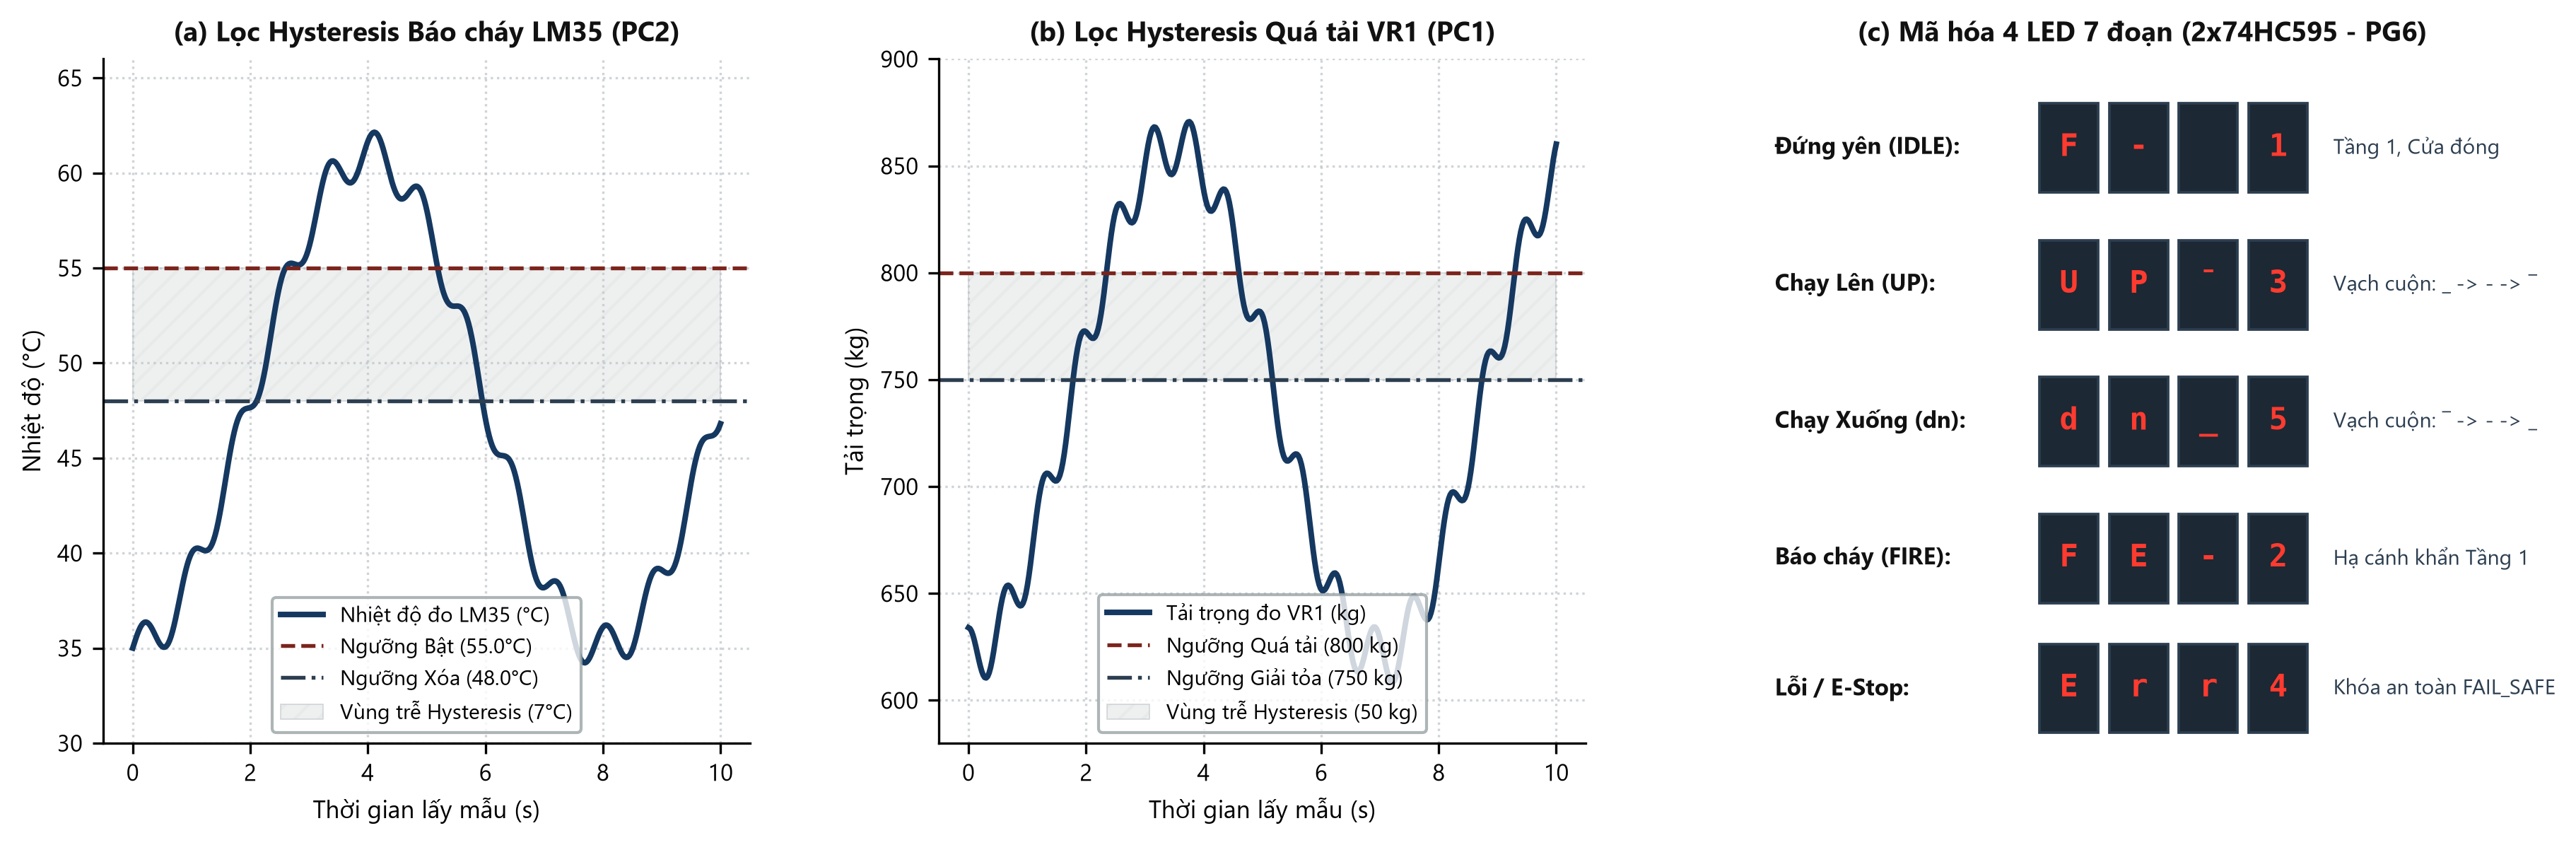
\includegraphics[width=0.99\textwidth]{image/fig_hysteresis_hmi.png}
\caption{Đồ thị đặc tuyến trễ 2 ngưỡng (Hysteresis) của \texttt{LM35} \& \texttt{VR1} và quy tắc mã hóa 4 LED 7 đoạn trên bus \texttt{SPI1}}
\label{fig:hysteresis_hmi}
\end{figure}

\begingroup
\renewcommand{\arraystretch}{1.18}%
\setlength{\tabcolsep}{4.5pt}%
\fontsize{8.2}{10.5}\selectfont
\arrayrulecolor{tableborder}%
\begin{xltabular}{\textwidth}{|C{2.0cm}|L{3.2cm}|L{3.5cm}|Y|}
\caption{Bảng ánh xạ chức năng 16 phím ma trận 4$\times$4 (\texttt{PD3}) và mã hiển thị 4 LED 7 đoạn (\texttt{PG6})}\label{tab:keypad_7seg}\\
\hline
\rowcolor{tablehead}
\thcell{Mã Phím} & \thcell{Sự kiện HSM phát sinh} & \thcell{Chức năng trên Bo mạch} & \thcell{Phản hồi Âm thanh (PF8) \& LED 7 Đoạn (PG6)} \\
\hline
\endfirsthead
\hline
\rowcolor{tablehead}
\thcell{Mã Phím} & \thcell{Sự kiện HSM phát sinh} & \thcell{Chức năng trên Bo mạch} & \thcell{Phản hồi Âm thanh (PF8) \& LED 7 Đoạn (PG6)} \\
\hline
\endhead
\hline
\endfoot
\hline
\endlastfoot
\texttt{Phím 0..6} & \texttt{EV\_CALL\_CABIN (1..7)} & Gọi trực tiếp \textbf{Tầng 1 .. Tầng 7}. & Còi bíp \texttt{2400 Hz (35 ms)}; đưa tầng vào \texttt{cabin\_mask}. \\
\hline
\rowcolor{roweven}
\texttt{Phím 7} & \texttt{EV\_DOOR\_OPEN\_REQ} & Nút \textbf{Mở cửa nhanh (\texttt{<|>})} tại tầng. & Còi bíp \texttt{2400 Hz}; mở lại cửa nếu đang đứng yên/đang đóng. \\
\hline
\texttt{Phím 8} & \texttt{EV\_DOOR\_CLOSE\_REQ} & Nút \textbf{Đóng cửa nhanh (\texttt{>|<})}. & Còi bíp \texttt{2400 Hz}; rút ngắn thời gian giữ mở cửa. \\
\hline
\rowcolor{roweven}
\texttt{Phím 9} & \texttt{EV\_DOOR\_OBSTRUCT\_X0} & Giả lập \textbf{Kẹt cửa (\texttt{X0 -- PA6})}. & Còi cảnh báo kép \texttt{1800 Hz}; đảo chiều mở cửa ngay lập tức. \\
\hline
\texttt{Phím 10} & \texttt{EV\_FIRE\_DETECTED} & Kích hoạt \textbf{Báo cháy khẩn cấp}. & Còi hụ báo cháy \texttt{2800/1800 Hz}; LED hiển thị \texttt{FE- [Tầng]}. \\
\hline
\rowcolor{roweven}
\texttt{Phím 11} & \texttt{EV\_ESTOP\_X1} & Kích hoạt \textbf{Dừng khẩn (\texttt{E-Stop})}. & Còi cảnh báo lỗi; cắt rơ-le \texttt{PE5/PE6}, LED hiển thị \texttt{Err[Tầng]}. \\
\hline
\texttt{Phím 12..15} & \texttt{EV\_FAULT\_CLEAR} & \textbf{Xóa lỗi / Khôi phục (\texttt{CLEAR})}. & Xóa trạng thái \texttt{FIRE\_EVAC / FAIL\_SAFE} về \texttt{IDLE\_CLOSED}. \\
\end{xltabular}
\endgroup

\pagebreak
Đoạn mã nguồn C dưới đây minh họa trực tiếp giải thuật quy đổi điện áp 5 kênh ADC sang các đại lượng vật lý chuẩn trong \texttt{bsp\_adc\_sensors.c} và thuật toán lọc trễ Hysteresis 2 ngưỡng kích hoạt cảnh báo an toàn trong luồng \texttt{t1\_safety}:

\begin{lstlisting}[language=C, caption={Quy đổi ADC 5 kênh (bsp\_adc\_sensors.c) và cơ chế Hysteresis trong t1\_safety (main.c)}]
/* 1. Quy doi dien ap ADC 12-bit sang dai do vat ly (zero-float) */
int bsp_adc_read(bsp_adc_data_t *out) {
    out->temp_deci_c = mv_vals[0]; /* LM35: 10 mV/C -> 0.1 C */
    int32_t load = (mv_vals[1] * (int32_t)ELEV_LOAD_MAX_KG) / 3300;
    out->load_kg = (uint16_t)CLAMP(load, 0, ELEV_LOAD_MAX_KG);
    out->light_mv   = (uint16_t)CLAMP(mv_vals[2], 0, 3300);
    out->bus_mv     = (uint16_t)CLAMP(mv_vals[3], 0, 3300);
    out->current_mv = (uint16_t)CLAMP(mv_vals[4], 0, 3300);
    return any_ok ? 0 : -EIO;
}

/* 2. Bo loc tre Hysteresis 2 nguong trong luong t1_safety */
/* Bao chay: Bat >=55.0 C (550), giai toa khi ha <=48.0 C (480) */
if (!prev_overheat && adc.temp_deci_c >= 550) {
    prev_overheat = true;
    elevator_event_t ev = { .type = EV_OVERHEAT_TEMP,
                            .param = adc.temp_deci_c };
    (void)elevator_hsm_post_event(&ev);
    (void)can_bus_send_emergency(1U, 0U);
} else if (prev_overheat &&
           adc.temp_deci_c <= ELEV_TEMP_CLEAR_THRESH_DC) {
    prev_overheat = false;
    elevator_event_t ev = { .type = EV_TEMP_NORMAL };
    (void)elevator_hsm_post_event(&ev);
}

/* Qua tai: Bat >=800 kg (giu cua), chi xoa khi tai <=750 kg */
if (!prev_overload && ((adc_ok && adc.load_kg >= 800) || x3)) {
    prev_overload = true;
    elevator_event_t ev = { .type = EV_OVERLOAD_SET,
                            .param = adc.load_kg };
    (void)elevator_hsm_post_event(&ev);
} else if (prev_overload && !x3 &&
           (!adc_ok || adc.load_kg <= ELEV_LOAD_CLEAR_KG)) {
    prev_overload = false;
    elevator_event_t ev = { .type = EV_OVERLOAD_CLEAR };
    (void)elevator_hsm_post_event(&ev);
}
\end{lstlisting}

\subsection{Giao thức CAN Bus 500 kbps, Bộ lọc Phần cứng và Cơ chế Fail-Safe}
Nhằm hiện thực hóa mạng truyền thông công nghiệp phân tán có khả năng kháng nhiễu điện từ cao giữa bộ điều khiển cabin và trạm hiển thị hành lang ngoài sảnh, lớp truyền thông tích hợp bộ điều khiển vi mô CAN 2.0A ở tốc độ 500 kbps kết hợp cơ chế tự phục hồi lỗi đường truyền (Hình~\ref{fig:can_eeprom}A và Bảng~\ref{tab:can_frames}):
\begin{itemize}[nosep]
    \item \textbf{Trình tự khởi tạo chuẩn theo Zephyr Driver và Phân bổ CAN ID ưu tiên (\textit{CSMA/AMP}):}
    \begin{itemize}[nosep]
        \item \textit{Trình tự khởi động driver:} Tuân thủ nghiêm ngặt chuỗi gọi hàm tiêu chuẩn của Zephyr CAN API: cấu hình chế độ hoạt động kèm cơ chế phục hồi thủ công qua \texttt{can\_set\_mode(can\_dev, mode | CAN\_MODE\_MANUAL\_RECOVERY)} $\rightarrow$ đăng ký 3 bộ lọc phần cứng vào hàng đợi \texttt{g\_can\_rx\_msgq} bằng \texttt{can\_add\_rx\_filter\_msgq()} $\rightarrow$ kích hoạt bộ điều khiển bằng \texttt{can\_start()}.
        \item \textit{3 bộ lọc chấp nhận phần cứng (Hardware Acceptance Filters):} Tận dụng cơ chế lọc mặt nạ trực tiếp trên thanh ghi của khối \texttt{bxCAN1} để loại bỏ 100\% các khung tin không thuộc phạm vi xử lý mà không làm tiêu tốn chu kỳ CPU:
        \begin{itemize}[nosep]
            \item \textbf{Filter 1 (Mask \texttt{0x7FF}):} Khớp chính xác duy nhất khung khẩn cấp \texttt{0x080} (Dừng khẩn / Báo cháy).
            \item \textbf{Filter 2 (Mask \texttt{0x7F0}):} Khớp dải 16 mã ID \texttt{0x100..0x10F} chuyên dùng nhận các lệnh gọi tầng từ sảnh ngoài.
            \item \textbf{Filter 3 (Mask \texttt{0x600}):} Khớp toàn bộ dải ID \texttt{0x200..0x3FF}, tiếp nhận đồng thời khung trạng thái cabin (\texttt{0x200}), khung nhịp tim Heartbeat định kỳ (\texttt{0x300}), khung kiểm tra độ trễ khứ hồi \texttt{canping} (\texttt{0x380/0x381}) và yêu cầu truyền từ xa (\texttt{RTR}).
        \end{itemize}
        \item \textit{Phân cấp ưu tiên không phá hủy:} Dựa trên đặc tính mức logic '0' có tính trạng thái trội (Dominant Bit) của chuẩn CAN 2.0A, các gói tin có CAN ID nhỏ hơn sẽ luôn chiếm quyền truyền dẫn tức thời. Khung sự cố an toàn (\texttt{0x080}) luôn chiếm ưu thế tuyệt đối trước khung dữ liệu định kỳ (\texttt{0x200/0x300}).
    \end{itemize}
    \item \textbf{Truyền bất đồng bộ kèm Callback, chuẩn hóa Big-Endian và Phản hồi khung \texttt{RTR}:}
    \begin{itemize}[nosep]
        \item Mọi thao tác phát khung tin qua \texttt{can\_send()} đều thiết lập hàm callback bất đồng bộ \texttt{can\_tx\_done\_cb()} với thời gian chờ tối đa 20 ms. Việc truyền diễn ra hoàn toàn không chặn (non-blocking), cập nhật số lượng khung thành công/thất bại qua hai biến đếm nguyên tử \texttt{g\_tx\_ok} và \texttt{g\_tx\_err}.
        \item Toàn bộ dữ liệu nhiều byte (\texttt{uptime\_ms} 32-bit, số thứ tự \texttt{seq} 16-bit, dấu thời gian đo độ trễ \texttt{RTT}) đều được mã hóa tường minh theo định dạng mạng \textbf{Big-Endian} (\texttt{sys\_put\_be32}, \texttt{sys\_put\_be16}), bảo đảm tính tương thích nhị phân tuyệt đối giữa STM32 Cortex-M4 (Little-Endian) và ứng dụng giám sát PC Digital Twin (x86\_64).
        \item Tùy chọn cấu hình \texttt{CONFIG\_CAN\_ACCEPT\_RTR=y} cho phép bộ điều khiển cabin phát hiện và phản hồi ngay lập tức khung trạng thái mới nhất khi trạm sảnh phát tín hiệu truy vấn từ xa \texttt{CAN\_FRAME\_RTR} trên ID \texttt{0x200}.
    \end{itemize}
    \item \textbf{Giám sát mất kết nối 2000~ms và Phục hồi tự động khỏi trạng thái \texttt{BUS-OFF}:}
    \begin{itemize}[nosep]
        \item \textit{Watchdog đối tác (\texttt{t3\_can\_wdt}):} Luồng chuyên trách ngủ trên lệnh nhận semaphore \texttt{k\_sem\_take(\&g\_can\_partner\_sem, K\_MSEC(2000))}. Khi đối tác mất nguồn hoặc cáp truyền thông bị đứt quá 2000 ms, hàm trả về lỗi \texttt{-EAGAIN}. Hệ thống chốt cờ lỗi đường truyền \texttt{g\_link\_fault\_latched}, hủy bỏ chế độ hiển thị từ xa và phát sự kiện \texttt{EV\_CAN\_LINK\_LOST} đưa thang máy vào trạng thái an toàn \texttt{HSM\_STATE\_FAIL\_SAFE}.
        \item \textit{Tự động thoát lỗi BUS-OFF:} Khi bộ đếm lỗi truyền \texttt{TEC} vượt quá ngưỡng 255 do đoản mạch hoặc xung nhiễu lớn, phần cứng tự động cô lập bộ thu phát (\texttt{CAN\_STATE\_BUS\_OFF}). Trong luồng \texttt{t3\_can\_tx}, hệ thống định kỳ kiểm tra trạng thái bus; nếu phát hiện \texttt{BUS-OFF}, hệ thống ghi mã sự cố \texttt{BB\_FAULT\_CAN\_BUS\_OFF} vào hộp đen EEPROM, giới hạn tần suất xử lý (tối đa 1 lần/giây) và kích hoạt hàm phục hồi Zephyr \texttt{can\_recover(can\_dev, K\_MSEC(100))} để kéo bộ điều khiển trở lại mạng.
    \end{itemize}
\end{itemize}

\begin{figure}[H]
\centering
\resizebox{\textwidth}{!}{%
\begin{tikzpicture}
    % === PHAN A: 3 BO LOC PHAN CUNG bxCAN1 (500 kbps) ===
    \node[font=\footnotesize\bfseries, text=tablehead, anchor=west] at (0, 5.75)
        {(a) Phân hoạch Ưu tiên 11-bit (\textit{CSMA/AMP}) và 3 Bộ lọc Chấp nhận Phần cứng \texttt{bxCAN1} (\texttt{500 kbps})};

    \node[acadbox, text width=4.85cm, minimum height=1.80cm] (F1) at (2.55, 4.40)
        {\textbf{HW Filter 1 -- Mức Khẩn cấp}\\[1pt]
         {\tiny \texttt{ID = 0x080 | Mask = 0x7FF}}\\[2pt]
         {\tiny Thắng phân xử bit tuyệt đối trên bus\\
         \texttt{DLC=2}: [\texttt{Mã E-Stop/Fire}, \texttt{Tầng}]}};

    \node[acadbox, text width=4.85cm, minimum height=1.80cm] (F2) at (7.90, 4.40)
        {\textbf{HW Filter 2 -- Gọi tầng Hành lang}\\[1pt]
         {\tiny \texttt{ID = 0x100..0x10F | Mask = 0x7F0}}\\[2pt]
         {\tiny Gom lệnh gọi nút \texttt{HALL} về \texttt{CABIN}\\
         \texttt{DLC=2}: [\texttt{Tầng 1..7}, \texttt{UP/DOWN}]}};

    \node[acadbox, text width=4.85cm, minimum height=1.80cm] (F3) at (13.25, 4.40)
        {\textbf{HW Filter 3 -- Giám sát \& Đo RTT}\\[1pt]
         {\tiny \texttt{ID = 0x200..0x3FF | Mask = 0x600}}\\[2pt]
         {\tiny \texttt{0x200} Status (\texttt{RTR}) $\cdot$ \texttt{0x300} HB \texttt{250ms}\\
         \texttt{0x380/0x381} Khung đo \texttt{PING/PONG}}};

    % === PHAN B: TO CHUC BO NHO AT24C512 EEPROM (64 KB, Trang 128 B) ===
    \node[font=\footnotesize\bfseries, text=tablehead, anchor=west] at (0, 2.75)
        {(b) Sơ đồ Ánh xạ Vùng nhớ Hộp đen Vòng 32 Bản ghi trên \texttt{AT24C512 EEPROM} (\texttt{I2C1 0x50}, Trang \texttt{128 Byte})};

    \node[acadboxnav, text width=4.25cm, minimum height=1.85cm] (HDR) at (2.25, 1.25)
        {\textbf{Khối Header Quản lý}\\[1pt]
         {\tiny Địa chỉ \texttt{0x0000} (16 Bytes)}\\[2pt]
         {\tiny \texttt{magic = 0x454C4556 ("ELEV")}\\
         \texttt{next\_seq}, \texttt{write\_idx}, \texttt{valid\_cnt}\\
         Toàn vẹn: \texttt{crc32\_ieee} (4 Bytes)}};

    \node[acadbox, text width=5.65cm, minimum height=1.85cm] (RING) at (7.80, 1.25)
        {\textbf{Hàng đợi Vòng 32 Bản ghi Sự cố}\\[1pt]
         {\tiny Địa chỉ \texttt{0x0080 + idx * 32} (\texttt{STRIDE = 32 B})}\\[2pt]
         {\tiny Gói \texttt{elevator\_blackbox\_rec\_t} (22 Bytes packed)\\
          Nằm gọn trang \texttt{128 B}, chống xé trang I2C}};

    \node[acadbox, text width=4.35cm, minimum height=1.85cm] (REC) at (13.45, 1.25)
        {\textbf{Cơ chế An toàn \& Phục hồi}\\[1pt]
         {\tiny Tự ghi hộp đen khi xảy ra:}\\[2pt]
         {\tiny $\bullet$ \texttt{IWDG Reset} (2500ms) qua \texttt{HWINFO}\\
         $\bullet$ \texttt{CAN\_LINK\_LOST} (>2000ms)\\
         $\bullet$ \texttt{BUS-OFF} $\rightarrow$ \texttt{can\_recover()}}};

    \draw[acadarr] (HDR.east) -- (RING.west);
    \draw[acadarr] (REC.west) -- (RING.east);

    % Thanh chi tiet tung truong cua 1 ban ghi 22-byte packed ben trong 32-byte stride
    \node[font=\tiny\bfseries, text=black!80, anchor=west] at (0, -0.35)
        {Chi tiết phân bổ trường bên trong 1 bản ghi \texttt{elevator\_blackbox\_rec\_t} (địa chỉ tương đối \texttt{+0x00 .. +0x15}):};

    \draw[acadline, fill=black!3] (0.0, -1.45) rectangle (2.1, -0.70);
    \node[align=center, font=\tiny] at (1.05, -1.07) {\texttt{+0..3} (4B)\\\texttt{seq}};

    \draw[acadline, fill=white] (2.1, -1.45) rectangle (4.3, -0.70);
    \node[align=center, font=\tiny] at (3.20, -1.07) {\texttt{+4..7} (4B)\\\texttt{uptime\_ms}};

    \draw[acadline, fill=black!3] (4.3, -1.45) rectangle (7.6, -0.70);
    \node[align=center, font=\tiny] at (5.95, -1.07) {\texttt{+8..14} (7B)\\Giờ \texttt{DS3231} (\texttt{Y,M,D,h,m,s})};

    \draw[acadline, fill=white] (7.6, -1.45) rectangle (9.5, -0.70);
    \node[align=center, font=\tiny] at (8.55, -1.07) {\texttt{+15} (1B)\\\texttt{fault\_code}};

    \draw[acadline, fill=black!3] (9.5, -1.45) rectangle (11.4, -0.70);
    \node[align=center, font=\tiny] at (10.45, -1.07) {\texttt{+16..17} (2B)\\\texttt{state}, \texttt{floor}};

    \draw[acadline, fill=white] (11.4, -1.45) rectangle (13.6, -0.70);
    \node[align=center, font=\tiny] at (12.50, -1.07) {\texttt{+18..19} (2B)\\\texttt{temp\_deci\_c}};

    \draw[acadline, fill=tablehead!12] (13.6, -1.45) rectangle (15.80, -0.70);
    \node[align=center, font=\tiny] at (14.70, -1.07) {\texttt{+20..21} (2B)\\\textbf{\texttt{crc16\_ccitt}}};
\end{tikzpicture}%
}

\caption{Kiến trúc 3 bộ lọc phần cứng \texttt{bxCAN 500 kbps} và cấu trúc vùng nhớ hộp đen vòng 32 bản ghi trên \texttt{AT24C512 EEPROM}}
\label{fig:can_eeprom}
\end{figure}

\begingroup
\renewcommand{\arraystretch}{1.18}%
\setlength{\tabcolsep}{4pt}%
\fontsize{8.1}{10.4}\selectfont
\arrayrulecolor{tableborder}%
\begin{xltabular}{\textwidth}{|C{1.45cm}|C{2.1cm}|C{1.1cm}|C{1.9cm}|Y|}
\caption{Đặc tả tập khung truyền mạng CAN Bus 500 kbps và cấu trúc Payload (Big-Endian)}\label{tab:can_frames}\\
\hline
\rowcolor{tablehead}
\thcell{CAN ID} & \thcell{Bộ lọc Phần cứng} & \thcell{DLC} & \thcell{Chu kỳ / Kiểu} & \thcell{Định dạng Byte Payload (Big-Endian) \& Ý nghĩa} \\
\hline
\endfirsthead
\hline
\rowcolor{tablehead}
\thcell{CAN ID} & \thcell{Bộ lọc Phần cứng} & \thcell{DLC} & \thcell{Chu kỳ / Kiểu} & \thcell{Định dạng Byte Payload (Big-Endian) \& Ý nghĩa} \\
\hline
\endhead
\hline
\endfoot
\hline
\endlastfoot
\texttt{0x080} & Filter 1 (\texttt{0x7FF}) & 3~B & Sự kiện khẩn & \texttt{B0}: Mã lỗi (\texttt{1=Fire, 2=E-Stop}); \texttt{B1}: Tầng; \texttt{B2}: \texttt{0xFF}. \\
\hline
\rowcolor{roweven}
\texttt{0x10x} & Filter 2 (\texttt{0x7F0}) & 2~B & Khi bấm gọi & \texttt{B0}: Tầng gọi (\texttt{1..7}); \texttt{B1}: Hướng gọi (\texttt{1=UP, 0=DOWN}). \\
\hline
\texttt{0x200} & Filter 3 (\texttt{0x600}) & 8~B & 250~ms / \texttt{RTR} & \texttt{B0}: State; \texttt{B1}: Tầng; \texttt{B2}: Đích; \texttt{B3}: Dir+1; \texttt{B4}: Cửa\%; \texttt{B5}: Flags; \texttt{B6..7}: Mask. \\
\hline
\rowcolor{roweven}
\texttt{0x300} & Filter 3 (\texttt{0x600}) & 8~B & 250~ms (Định kỳ) & \texttt{B0}: Role (\texttt{0xA5/0x5A}); \texttt{B1}: State; \texttt{B2..5}: \texttt{uptime\_ms} (BE32); \texttt{B6..7}: \texttt{seq} (BE16). \\
\hline
\texttt{0x380} & Filter 3 (\texttt{0x600}) & 8~B & Lệnh \texttt{canping} & Khung \textbf{PING} chứa \texttt{seq} (\texttt{BE32}) và \texttt{uptime\_ms} (\texttt{BE32}). \\
\hline
\rowcolor{roweven}
\texttt{0x381} & Filter 3 (\texttt{0x600}) & 8~B & Phản hồi tức thời & Khung \textbf{PONG} hoàn trả payload để tính độ trễ khứ hồi \texttt{RTT} qua DWT. \\
\end{xltabular}
\endgroup

\pagebreak
Đoạn mã nguồn C trích từ \texttt{src/comms/can\_bus.c} dưới đây minh họa chi tiết quá trình thiết lập 3 bộ lọc phần cứng trên bộ điều khiển \texttt{bxCAN1}, vòng lặp giám sát liên kết truyền thông 2000~ms và cơ chế tự động phục hồi khỏi lỗi \texttt{BUS-OFF}:

\begin{lstlisting}[language=C, caption={Cấu hình 3 bộ lọc phần cứng (can\_bus.c) và giám sát liên kết CAN 2000~ms (t3\_can\_wdt)}]
/* 1. Cai dat 3 bo loc chap nhan phan cung tren bxCAN1 */
static int install_hw_filters(void) {
    /* Filter 1: 0x080 E-Stop (mask 0x7FF) */
    const struct can_filter f1 = {
        .id = CAN_ID_EMERGENCY_STOP, .mask = 0x7FFU
    };
    /* Filter 2: 0x100..0x10F Hall Calls (mask 0x7F0) */
    const struct can_filter f2 = {
        .id = CAN_ID_HALL_CALL, .mask = 0x7F0U
    };
    /* Filter 3: 0x200..0x3FF Cabin Status (mask 0x600) */
    const struct can_filter f3 = {
        .id = CAN_ID_CABIN_STATUS, .mask = 0x600U
    };
    int id1 = can_add_rx_filter_msgq(can_dev, &g_can_rx_msgq, &f1);
    int id2 = can_add_rx_filter_msgq(can_dev, &g_can_rx_msgq, &f2);
    int id3 = can_add_rx_filter_msgq(can_dev, &g_can_rx_msgq, &f3);
    return (id1 >= 0 && id2 >= 0 && id3 >= 0) ? 0 : -ENOSPC;
}

/* 2. Giam sat nhip tim doi tac voi timeout 2000 ms (t3_can_wdt) */
void can_bus_partner_watchdog_step(void) {
    int err = k_sem_take(&g_can_partner_sem,
                         K_MSEC(ELEV_CAN_TIMEOUT_MS));
    if (err == -EAGAIN) { /* Qua 2000 ms mat heartbeat */
        k_mutex_lock(&g_can_state_mutex, K_FOREVER);
        bool first_fault = !g_link_fault_latched;
        if (first_fault) {
            g_link_fault_latched = true;
            g_remote_valid = false;
        }
        k_mutex_unlock(&g_can_state_mutex);
        if (first_fault) {
            elevator_event_t ev = { .type = EV_CAN_LINK_LOST };
            (void)elevator_hsm_post_event(&ev);
        }
    }
}

/* 3. Phat hien BUS-OFF, ghi hop den va can_recover() */
if (state == CAN_STATE_BUS_OFF &&
    (now_ms - g_last_recover_ms) > 1000U) {
    g_last_recover_ms = now_ms;
    LOG_ERR("CAN BUS-OFF (TEC=%u) -> recover", cnt.tx_err_cnt);
    (void)bsp_blackbox_append(BB_FAULT_CAN_BUS_OFF,
                              HSM_STATE_FAIL_SAFE, 0U, 0);
    (void)can_recover(can_dev, K_MSEC(100));
}
\end{lstlisting}

\subsection{Hộp đen EEPROM AT24C512, Hardware Watchdog và Kết quả Biên dịch}
Nhằm đảm bảo khả năng tự giám sát độ sống của toàn bộ các luồng phần mềm, lưu trữ bất khả biến các biến cố an toàn và đánh giá hiệu năng tối ưu tài nguyên của hệ thống, firmware tích hợp bộ đếm Independent Watchdog, hệ thống hộp đen EEPROM hai tầng kiểm tra toàn vẹn và thực hiện đo lường bộ nhớ lúc biên dịch (Hình~\ref{fig:can_eeprom}B và Bảng~\ref{tab:eeprom_layout}):
\begin{itemize}[nosep]
    \item \textbf{Giám sát độ sống đa luồng qua Hardware Watchdog (\textmd{\texttt{IWDG}}) và Định danh nguyên nhân khởi động:}
    \begin{itemize}[nosep]
        \item \textit{Nguyên tắc điểm danh đa luồng (\texttt{bsp\_wdt\_checkin}):} Bộ đếm thời gian độc lập IWDG trên STM32F407 vận hành từ nguồn xung nội bộ LSI ($\sim 32\text{ kHz}$) độc lập hoàn toàn với mạch dao động chính, với ngưỡng tràn ngắt cứng là 2500 ms. Để ngăn ngừa hiện tượng một luồng đơn lẻ còn chạy tiếp tục nuôi watchdog trong khi các luồng khác đã bị treo chết (deadlock), hệ thống thiết lập cơ chế kiểm tra chéo: cả 4 luồng trọng yếu (\texttt{t1\_safety}, \texttt{t2\_fsm}, \texttt{t3\_can\_tx}, \texttt{t4\_hmi}) đều bắt buộc phải định kỳ gọi hàm \texttt{bsp\_wdt\_checkin(id)} để cập nhật mốc thời gian sống.
        \item \textit{Dịch vụ nạp Watchdog (\texttt{bsp\_wdt\_service}):} Luồng giám sát \texttt{t5\_wdt} định kỳ mỗi 100 ms quét mảng mốc thời gian của 4 luồng dưới sự bảo vệ của khóa quay \texttt{k\_spinlock} (\texttt{g\_wdt\_lock}). Chỉ khi toàn bộ 4 luồng đều có thời gian phản hồi trong vòng \texttt{THREAD\_STALL\_TIMEOUT\_MS = 1500 ms} gần nhất, hàm mới thực thi lệnh \texttt{wdt\_feed()}. Nếu bất kỳ luồng nào bị treo quá 1500 ms, lệnh nạp bị khóa hoàn toàn, buộc phần cứng kích hoạt reset hệ thống sau đúng 2500 ms.
        \item \textit{Định danh nguyên nhân khởi động qua \texttt{HWINFO}:} Ngay khi CPU khởi động lại, hàm \texttt{bsp\_watchdog\_init} kiểm tra cờ nguyên nhân qua \texttt{hwinfo\_get\_\allowbreak reset\_\allowbreak cause()}. Nếu phát hiện cờ \texttt{RESET\_\allowbreak WATCHDOG} (do IWDG kích hoạt), firmware lập tức ghi bản ghi sự cố \texttt{BB\_FAULT\_\allowbreak BOOT\_\allowbreak WATCHDOG} vào hộp đen EEPROM rồi gọi \texttt{hwinfo\_clear\_\allowbreak reset\_\allowbreak cause()}, giúp phân biệt rạch ròi giữa khởi động cấp nguồn và khởi động khôi phục lỗi treo.
    \end{itemize}
    \item \textbf{Hộp đen vòng 32 bản ghi trên AT24C512 EEPROM với IC thời gian thực DS3231:}
    \begin{itemize}[nosep]
        \item \textit{Phần cứng lưu trữ chuyên dụng:} Hệ thống khai thác chip nhớ EEPROM I2C \textbf{AT24C512} (dung lượng 64 KB, tổ chức theo trang vật lý 128 Byte) kết hợp chip đồng hồ thời gian thực \textbf{DS3231} (độ chính xác $\pm 2\text{ ppm}$, có pin CMOS dự phòng) trên cùng bus \texttt{I2C1} được bảo vệ bởi khóa kế thừa độ ưu tiên \texttt{g\_i2c1\_bus\_mutex}.
        \item \textit{Cấu trúc bản ghi và Căn chỉnh trang an toàn:} Mỗi bản ghi sự cố \texttt{elevator\_\allowbreak blackbox\_\allowbreak rec\_t} có kích thước nén 22 Byte và bước nhảy địa chỉ cố định \texttt{BB\_REC\_STRIDE = 32 Bytes}. Vùng nhớ 32 bản ghi (địa chỉ \texttt{0x0080..0x047F}) được thiết kế sao cho mỗi trang 128 Byte của EEPROM chứa trọn vẹn đúng 4 bản ghi, triệt tiêu hoàn toàn rủi ro ghi tràn biên trang vật lý (Page-boundary Wrap-around).
        \item \textit{Toàn vẹn dữ liệu hai tầng (\textit{Two-Tier Integrity}):} Khối thông tin đầu trang (\textit{Header}) tại \texttt{0x0000} quản lý \texttt{magic} (\texttt{0x424B4954}), con trỏ ghi xoay vòng \texttt{write\_idx}, số bản ghi hợp lệ \texttt{valid\_count} và số thứ tự đơn điệu \texttt{next\_seq}, được bảo vệ bởi mã băm kiểm tra \textbf{CRC32-IEEE}. Từng bản ghi sự cố tại \texttt{0x0080 + idx * 32} lưu trữ đầy đủ dấu thời gian thực (Năm, Tháng, Ngày, Giờ, Phút, Giây), mã lỗi, trạng thái HSM, tầng và nhiệt độ, được bảo vệ riêng bằng mã \textbf{CRC16-CCITT} (đa thức \texttt{0x1021}).
        \item \textit{Quy trình ghi bất đối xứng an toàn mất điện:} Firmware luôn ghi toàn bộ cấu trúc bản ghi mới xuống vùng nhớ ô dữ liệu trước; chỉ khi giao dịch I2C thành công mới cập nhật con trỏ \texttt{write\_idx} và tính lại \texttt{CRC32} ghi xuống Header, đảm bảo dữ liệu lịch sử không bao giờ bị hỏng nếu nguồn điện đột ngột bị ngắt giữa chừng.
    \end{itemize}
    \item \textbf{Kết quả biên dịch thực tế trên Zephyr SDK v1.0.1 (arm-zephyr-eabi-gcc 14.3.0):}
    \begin{itemize}[nosep]
        \item \textit{Độ tin cậy mã nguồn:} Toàn bộ 18 mục tiêu (bao gồm cả nhân Zephyr, driver BSP, máy trạng thái Core, mạng CAN và giao diện dòng lệnh CLI) đều được biên dịch thành công tuyệt đối: \textbf{0 lỗi (\texttt{0 errors}), 0 cảnh báo (\texttt{0 warnings})} ở mức cờ cảnh báo cao nhất \texttt{-Wall -Wextra}.
        \item \textit{Bộ nhớ chương trình (Flash ROM):} Chiếm dụng \textbf{104\,112 Bytes} trên tổng số 1\,048\,576 Bytes khả dụng (\textbf{9.93\%}), để lại hơn 900 KB dự phòng cho việc mở rộng thuật toán điều phối đa cabin và nạp firmware qua mạng (OTA).
        \item \textit{Bộ nhớ dữ liệu tĩnh (SRAM):} Chiếm dụng \textbf{28\,608 Bytes} trên tổng số 131\,072 Bytes (\textbf{21.83\%}). Toàn bộ 100\% biến nhớ và ngăn xếp luồng RTOS đều được cấp phát tĩnh lúc biên dịch (Zero Heap Dynamic Allocation), triệt tiêu hoàn toàn lỗi tràn bộ nhớ hoặc phân mảnh RAM trong các chu kỳ vận hành dài hạn.
    \end{itemize}
\end{itemize}

\begingroup
\renewcommand{\arraystretch}{1.18}%
\setlength{\tabcolsep}{4.5pt}%
\fontsize{8.2}{10.5}\selectfont
\arrayrulecolor{tableborder}%
\begin{xltabular}{\textwidth}{|C{2.0cm}|L{3.1cm}|C{2.1cm}|Y|}
\caption{Cấu trúc bản ghi sự cố (\texttt{elevator\_blackbox\_rec\_t}, bước 32-Byte) trên \texttt{AT24C512 EEPROM}}\label{tab:eeprom_layout}\\
\hline
\rowcolor{tablehead}
\thcell{Offset Byte} & \thcell{Tên Trường} & \thcell{Kiểu Dữ liệu} & \thcell{Mô tả Kỹ thuật \& Cơ chế Kiểm tra Toàn vẹn} \\
\hline
\endfirsthead
\hline
\rowcolor{tablehead}
\thcell{Offset Byte} & \thcell{Tên Trường} & \thcell{Kiểu Dữ liệu} & \thcell{Mô tả Kỹ thuật \& Cơ chế Kiểm tra Toàn vẹn} \\
\hline
\endhead
\hline
\endfoot
\hline
\endlastfoot
\texttt{Byte +0..+3} & \texttt{seq} & \texttt{uint32\_t} & Số thứ tự bản ghi tăng dần đơn điệu dùng để khôi phục thứ tự vòng đệm. \\
\hline
\rowcolor{roweven}
\texttt{Byte +4..+7} & \texttt{uptime\_ms} & \texttt{uint32\_t} & Thời gian hoạt động liên tục tính bằng mili-giây từ lúc MCU cấp nguồn. \\
\hline
\texttt{Byte +8..+14} & \texttt{year..sec} & \texttt{uint16\_t+5B} & Dấu thời gian thực (Năm, Tháng, Ngày, Giờ, Phút, Giây) đọc từ IC \textbf{DS3231} (\texttt{0x68}). \\
\hline
\rowcolor{roweven}
\texttt{Byte +15..+17} & \texttt{fault, state, floor} & \texttt{uint8\_t[3]} & Mã sự cố (\texttt{FIRE, OVERLOAD, OBSTRUCT, ESTOP, CAN\_LOST, WDT}), HSM state \& Tầng. \\
\hline
\texttt{Byte +18..+19} & \texttt{temp\_deci\_c} & \texttt{int16\_t} & Nhiệt độ cảm biến \texttt{LM35 (PC2)} tại thời điểm xảy ra sự cố (đơn vị $0.1^\circ\text{C}$). \\
\hline
\rowcolor{roweven}
\texttt{Byte +20..+21} & \texttt{crc16} & \texttt{uint16\_t} & Mã kiểm tra \textbf{CRC16-CCITT} (đa thức \texttt{0x1021}) tính trên 20 byte đầu của bản ghi. \\
\end{xltabular}
\endgroup

\pagebreak
Đoạn mã nguồn C trích từ \texttt{src/bsp/bsp\_watchdog.c} và \texttt{src/bsp/bsp\_i2c\_storage.c} sau đây minh họa thuật toán điểm danh 4 luồng trước khi nạp IWDG phần cứng và kỹ thuật ghi hộp đen xoay vòng bảo đảm toàn vẹn khi mất điện:

\begin{lstlisting}[language=C, caption={Dịch vụ Watchdog đa luồng (bsp\_watchdog.c) và ghi hộp đen an toàn (bsp\_i2c\_storage.c)}]
/* 1. Kiem tra 4 luong truoc khi nap IWDG (bsp_watchdog.c) */
bool bsp_wdt_service(bool force_freeze) {
    if (force_freeze || !g_wdt_ready) { return false; }
    int64_t now = k_uptime_get();
    k_spinlock_key_t key = k_spin_lock(&g_wdt_lock);
    for (size_t i = 0; i < WDT_MON_COUNT; i++) {
        if ((now - g_last_checkin_ms[i]) > 1500) {
            k_spin_unlock(&g_wdt_lock, key);
            LOG_ERR("WDT STALL: %s", bsp_wdt_slot_name(i));
            return false;
        }
    }
    k_spin_unlock(&g_wdt_lock, key);
    return (wdt_feed(wdt_dev, g_wdt_channel_id) == 0);
}

/* 2. Ghi hop den vong 32 ban ghi vao AT24C512 EEPROM (I2C1) */
int bsp_blackbox_append(blackbox_fault_code_t code,
                        elevator_state_t state,
                        uint8_t floor, int32_t temp_deci_c) {
    struct bb_header hdr = { 0 };
    elevator_blackbox_rec_t rec = { 0 };
    (void)bsp_rtc_get_datetime(&rec.year, &rec.month, &rec.day,
                               &rec.hour, &rec.min, &rec.sec);
    rec.seq = hdr.next_seq++; rec.fault_code = (uint8_t)code;
    rec.state = (uint8_t)state; rec.floor = floor;
    rec.temp_deci_c = (int16_t)temp_deci_c;
    rec.crc16 = bb_rec_crc(&rec); /* CRC16 tren 20 byte */

    k_mutex_lock(&g_i2c1_bus_mutex, K_FOREVER);
    off_t off = (off_t)(BB_REC_BASE_OFFSET +
                        hdr.write_idx * BB_REC_STRIDE);
    int err = eeprom_write(eeprom_dev, off, &rec, sizeof(rec));
    if (err == 0) {
        hdr.write_idx = (uint16_t)((hdr.write_idx + 1U) % 32U);
        hdr.crc32 = bb_hdr_crc(&hdr); /* CRC32 */
        err = eeprom_write(eeprom_dev, BB_HDR_OFFSET, &hdr, sizeof(hdr));
    }
    k_mutex_unlock(&g_i2c1_bus_mutex);
    return err;
}
\end{lstlisting}
